% 
\section{Introduction}
\label{sec:introduction}

In this paper, we investigate \emph{tiebreaking strategies} for cost-optimal \astar.
% In optimal search, tiebreaking strategies does not affect the optimality
% of the search algorithms because they only affect the node expansion
% order among the nodes with the same $f$-cost.
% \subsection{Tiebreaking for \astar}
% This paper is organized as follows.
% After defining some notations in \refsec{sec:preliminaries}, 
% We first investigate the conventional
% tiebreaking strategies for the optimal search using \astar.
\astar is the standard search algorithm for finding an optimal-cost path from an initial state $s$ to some goal
state $g \in G$ in a search space represented as a graph \cite{hart1968formal}.
It expands the nodes in the best-first order of $f(n)$ until up to $f^*$,
where $f(n)$ is a lower bound of the cost of the shortest path that contains a node $n$ and $f^*$ is the optimal cost.
% 
In many combinatorial search problems, the size of the last layer $f(n)=f^*$ of the search , called \emph{final plateau},
accounts for a significant fraction of the effective search space of \astar.  \refig{fig:plateau-noh}
(\refpage{fig:plateau-noh}) compares the number of states in this final plateau with $f(n) = f^*$ (y-axis)
vs. $f(n) \leq f^*$ (x-axis) for 1104 problem instances from the International Planning Competition (IPC1998-2011).
For many instances, a large fraction of the nodes in the effective search space have $f(n)=f^*$: The points
are located very close to the diagonal line ($x=y$), indicating almost all states with $f(n) \leq f^*$ have cost
$f^*$.

\refig{fig:plateau-0} depicts the conceptual view of these phenomenon.
% 
A naive view of the search space (left) would consider the space searched by \astar as
a thin layer of final plateau $f(n)=f^*$ surrounding a large number of closed nodes with $f<f^*$.  This view is
intuitive, and may accurately describe some real, practical search spaces such as 2D path finding on an explicit
graph. It also gives a foundation to some family of search algorithms like Frontier Search
\cite{korf1999divide,korf2000divide}, which tries to reduce the memory requirement by discarding the information on
$f<f^*$, which may work if $f<f^*$ is large.
% 
However, for many combinatorial search problems,
the figure on the right is a more accurate depiction -- the  search space has a large plateau for $f=f^*$.
In fact, Iterative Deepening approaches \cite{korf1985depth} assume this type of search space
where this final frontier is quite huge and the cost of re-evaluating $f<f^*$ is limited.
Classical planning problems in IPC benchmarks are clearly the instances of such combinatorial search problems.
\todo*{The fact that the last layer of search dominates the search was the motivation for Frontier Search and its numerous variants, so the SoCS community has been well aware of this --- SoCS community considers the opposite. Frontier search would not gain advantage in the planning domains because the number of nodes being forgotten is low compared to the size of the plateau.}

\begin{figure}[htbp]
  \centering
  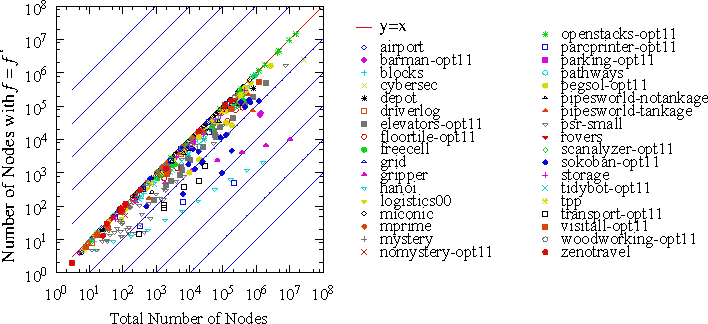
\includegraphics{tables/aaai16-frontier/aaai16prelim3/lmcut_frontier_noh-front.pdf}
 \caption{
 The number of nodes with $f=f^*$ (y-axis) compared to the
 total number of nodes in the search space (x-axis) with $f\leq f^*$ on 1104 IPC benchmark problems.
 This experiment uses a modified Fast Downward with \lmcut which 
 continues the search within the current $f$ after any optimal solution is found.
 This effectively generates all nodes with cost $f^*$.
  }
 \label{fig:plateau-noh}
\end{figure}

\begin{figure}[htbp]
  \centering
  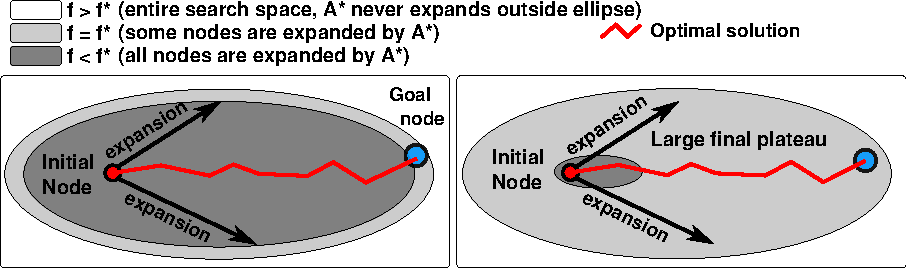
\includegraphics{img/astar/plateau-0.pdf}
 \caption{(Left) Naive understanding of the search space of \astar, which only holds for some limited domains. (Right) The reality of search spaces of combinatorial problems. Plateau containing the optimal goals ($f=f^*$) is large, and it even accounts for most of the search effort required by \astar.
  }
 \label{fig:plateau-0}
\end{figure}

In the majority of such IPC problem domains where the 
the last layer ($f(n)=f^*$) accounts for a significant fraction of the effective search space, a
\emph{tiebreaking strategy}, which determines which node to expand among nodes with the same $f$-cost,
can have a significant impact on the performance of \astar.
It is widely believed that among nodes with the same $f$-cost,
ties should be broken according to $h(n)$, i.e.,
nodes with smaller $h$-values should be expanded first.  While this is a
useful rule of thumb in many domains, it turns out that tiebreaking
requires more careful consideration, particularly for problems where
most or all of the nodes in the last layer have the same $h$-value.

We empirically evaluate the existing, commonly used, standard
tiebreaking strategies for \astar (\refsec{sec:eval-common-strategies}).
We show that:

\begin{enumerate}
 \item A Last-In-First-Out (\lifo) criterion tends to be more efficient
       than a First-In-First-Out (\fifo) criterion.
 \item Tiebreaking according to the heuristic value $h$, which
       frequently appears in the heuristic search literature, has little
       impact on the performance as long as \lifo default criterion is used 
       --  in other words, a \lifo tiebreaking policy is sufficient for most IPC domains.
 \item There are significant performance differences among tiebreaking strategies
       when domains include zero-cost actions. This is true even when $h$-based tiebreaking is used.
\end{enumerate}

While there are relatively few domains with zero-cost actions in the IPC
benchmark set, we argue that zero-cost actions naturally occur in
practical cost-minimization problems. Therefore we introduce a new set of
benchmarks called \emph{zerocost domains}
(\refsec{sec:zerocost-domains}).  We empirically show that these
zerocost domains have the different search space structure and different
problem difficulty from those of the original domains.

In order to solve such problems more efficiently, we propose and
evaluate \emph{depth diversification}, a new
tiebreaking method based on the notion of a node's \emph{depth} within a plateau,
which corresponds to the number of steps from the ``entrance'' to
the plateau (\refsec{sec:depth},
\refsec{sec:depth-based-evaluation}). We also evaluate an
admissible tiebreaking strategy which uses the distance-to-go estimate, a heuristic function which treats every actions
to have the unit costs (\refsec{sec:distance-to-go}).
Although distance-to-go estimates are inadmissible,
it does not harm the admissibility of entire search as long as it is used only for tiebreaking.
% 
In these sections, we empirically show that:
\begin{enumerate}
 \item Our new depth-based diversification strategy significantly improves upon the 
       standard tiebreaking strategies.
 \item Tiebreaking using distance-to-go variations of \lmcut, \mands and \ff heuristics
       significantly improves the standard tiebreaking strategies.
       \todo*{listing 3 points regarding d2go might give the wrong impression that this paper is about d2go. combine some of the d2go bullets, or add another depth-related bullet?}
 % \item Distance-to-go variations of \emph{inadmissible} heuristics
 %       (\ff) further improves the performance by an order of magnitude.
 \item Combining depth-based diversification with distance-to-go heuristics 
       further improves the performance.
\end{enumerate}

Finally, in \refsec{sec:discussion}, we discuss the implications of these results.
We offer a new perspective to admissible \astar search:
Admissible \astar can be seen as a series of satisficing searches on each plateau,
and thus the problem of tiebreaking can be reduced to satisficing search techniques.
% 
In order to strengthen the connection between tiebreaking and satisficing search,
we also show a preliminary result of the depth diversification,
which was shown to improve tiebreaking performance,
also improves satisficing search using Greedy Best First Search (GBFS).
We further discuss the future direction, related works, and close the article.

\textbf{
Note for reviewers:
This paper is a significantly extended version of the AAAI-16 paper by
the same authors. The addition to the conference paper is the following:
\begin{enumerate}
 \item Introduction of deterministic depth-based diversification
       strategy (as opposed to the randomized version in the conference
       paper), and its theoretical analysis in \refsec{sec:depth}. We
       also added thorough empirical analysis in
       \refsec{sec:depth-based-evaluation} that are not included in the
       conference version.
 \item Empirical analysis of distance-to-go estimates in
       \refsec{sec:distance-to-go}.  Also, we included an empirical
       evaluation of the use of inadmissible FF heuristics as part of
       tiebreaking criterion, and its combination with the
       depths metric thereof.
 \item New perspective to \astar and the preliminary results on the use
       of depth for satisficing search (\refsec{sec:discussion}).
\end{enumerate}
}


% \section{Preliminaries and Definitions}

\label{sec:preliminaries}

We first define some notation and the terminology used throughout the
rest of the paper.
$h(n)$ denotes the estimate of the cost from the current node $n$ to the nearest goal node.
$g(n)$ is the current shortest path cost from the initial node to the
current node.
$f(n)=g(n)+h(n)$ is the estimate of the resulting cost of the path to a goal
containing the current node.
We omit the argument $(n)$ unless necessary.

A \emph{sorting strategy} for a best first search algorithm 
which tries to select a single node from the OPEN list.
Each sorting strategy is denoted as a vector of several \emph{sorting criteria}, such as
[$\text{criterion}_1$, $\text{criterion}_2$, $\ldots$,
$\text{criterion}_k$], which means: From the OPEN list, first, select a
set of nodes using $\text{criterion}_1$.  If there are still multiple
nodes remaining in the set, then break ties using $\text{criterion}_2$
and so on, until a single node is selected.  The \emph{first-level
sorting criterion} of a strategy is $\text{criterion}_1$, the
\emph{second-level sorting criterion} is $\text{criterion}_2$, and so on.
%% the word frontier is no longer used in the later text.
% \emph{final frontier} is the set of open nodes with $f^*$.
Note that this corresponds to the command line option format of Fast
Downward \cite{Helmert2006}.

Using this notation, \astar without any tiebreaking strategy can be
denoted as a Best-First Search (BFS) with $[f]$, and \astar which breaks ties according to $h$
value is denoted as $[f,h]$. Similarly, GBFS is denoted as 
$[h]$.  Unless stated otherwise, we assume the nodes are sorted in the
increasing order of the key value, and a BFS always selects the smallest
key value.

The sorting strategy may fail to select a single node because some nodes
may share the same sorting keys. In such cases, a search algorithm must
decide which node to expand by a \emph{default} tiebreaking
strategy $\text{criterion}_k$ such as  \fifo (first-in-first-out), \lifo
(last-in-first-out) or \ro (random ordering).  
By definition, there is only 1 node which satisfies these criteria, so these
strategies are able to select a single node from the set of
nodes. Although these default strategies may not be a ``sorting''
criterion, {\bf [XXX - why?]}
 we also include them in the vector notation. For
example, an \astar using \fifo tiebreaking is denoted as $[f,h,\fifo]$.


Given a search algorithm which uses a particular sorting strategy, 
a \emph{plateau} is a set of nodes in OPEN whose elements are
indistinguishable according to the sorting strategy. In a case of \astar
using tiebreaking with $h$ ($[f,h]$), this is the set of nodes with the
same $f$ cost and the same $h$ cost.
A plateau whose nodes have $f=f_p$ and $h=h_p$ is denoted as $\plateau{f_p,h_p}$.

An \emph{entrance} to a $\plateau{f_p,h_p}$ is a node $n \in
\plateau{f_p,h_p}$, whose current parent is not a member of
$\plateau{f_p,h_p}$.  The \emph{final plateau}, is the plateau
containing the solution found by the search algorithm.  In \astar using
admissible heuristics, the final plateau is $\plateau{f^*}$ (without
tiebreaking), or $\plateau{f^*,0}$ (with $h$-based tiebreaking).

% \section{Background: Tiebreaking Strategies for \astar}

\label{sec:astar-background}

\astar is a standard search algorithm for finding an optimal cost path
on a graph.
Starting from the single initial node, in each iteration, \astar
selects and expands a node $n$ with the lowest $f$-cost in the OPEN
priority queue. The successor nodes are inserted back to OPEN, and $n$
is marked as CLOSED, in order to avoid duplicated evaluations.
\astar returns an optimal solution when $h$ is admissible, i.e., when
$\forall n; h(n) \leq h^*(n)$, where $h^*(n)$ is the optimal distance from $n$ to
the nearest goal.

The best-first order of the expansion is a key to guaranteeing solution optimality. 
The first solution found by the algorithm is guaranteed to have the optimal cost $f=f^*$ because 
all nodes with $f(n) < k$ are already expanded when it starts expanding
the nodes with $f(n) = k$.
Thus, the \emph{effective search space of \astar} is the set of nodes with 
$f(n) \leq f^*$: \astar expands all nodes with $f(n) < f^*$, then
expands \emph{some} of the nodes with $f(n) = f^*$, and
never expands the nodes with $f(n) > f^*$.

If there are multiple nodes with the same $f$-cost, \astar
must implement some tiebreaking strategy (either
explicitly or implicitly) which selects from among these nodes.
The early literature on heuristic search seems to have been mostly agnostic regarding tiebreaking.
The original \astar paper, as well as Nilsson's subsequent textbook 
states: ``Select the open node $n$ whose value $f$
is smallest. Resolve ties arbitrarily, but always in favor of any [goal
node]'' \cite[p.102 Step 2]{hart1968formal}, \cite[p.69]{Nilsson71}.
% Although it is possible to interpret this to imply $h$-based tiebreaking
% since goal nodes are the special case where $h=0$,
% they make no further mention of tiebreaking.
Pearl's textbook on heuristic search specifies that best-first search should ``break ties arbitrarily'' (\citeyear{pearl1984heuristics}, p.48, Step 3), and does not specifically mention tiebreaking for \astar.
To the best of our knowledge, the first explicit mention of a tiebreaking strategy that considers node generation order is by Korf in his analysis of IDA*: ``If \astar employs the tiebreaking rule of 'most-recently generated', it must also expand the same nodes [as IDA*]'', i.e., a \lifo ordering.

In recent years, tiebreaking according to $h$-values has become ``folklore'' in the search community.
\citeauthor{hansen2007anytime} state that ``[i]t is well-known 
that \astar achieves best performance when it breaks ties
in favor of nodes with least h-cost'' \cite{hansen2007anytime}.
\citeauthor{holte2010common} writes ``\astar breaks ties in favor
of larger $g$-values, as is most often done'' \cite[note that since $f=g+h$,
preferring large $g$ is equivalent to preferring smaller $h$]{holte2010common}.
\shortciteauthor{felner2011inconsistent} also assume ``ties are broken in
favor of low h-values'' in describing Bidirectional Pathmax for \astar \citeyear{felner2011inconsistent}.
In their detailed survey/tutorial on efficient \astar implementations,
\shortciteauthor{burns2012implementing} \citeyear{burns2012implementing}
also break ties ``preferring high $g$'' (equivalent to low $h$).
%% this could be moved to later analysis
% They further write: ``The reasoning is that the goal can be found more
% quickly in the final $f$ layer of search''.
Thus, tiebreaking according to $h$-values appears
to be ubiquitous in practice while,
to our knowledge, an in-depth experimental analysis of tiebreaking strategies for \astar is lacking in the literature.

Although the standard practice of tiebreaking according to $h$ might be
sufficient in some domains, further levels of tiebreaking (explicit or
implicit) are required if multiple nodes have the same $f$ as well as
the same $h$ values. To date, the effect of such \emph{default}
tiebreaking was not investigated in depth.
% 
For example, the survey of efficient \astar implementation techniques in
\cite{burns2012implementing} did not explicitly mention the default
tiebreaking, while their library
code\footnote{https://github.com/eaburns/search} uses \lifo
default tiebreaking.
% 
It first breaks ties according to $h$, and then
breaks remaining ties according to a \lifo criterion (most recently
generated nodes first), i.e., $[f,h,\lifo]$.
% 
Although not documented, their choice of a \lifo 2nd-level tiebreaking
criterion appears to be a natural consequence of the fact it can be
trivially and efficiently implemented in their two-level bucket (vector)
implementation of OPEN.
% 
In contrast, the current implementation of the \sota \astar based planner Fast
Downward \cite{Helmert2006}, as well as the work by \cite{RogerH10} uses
a $[f,h,\fifo]$ tiebreaking strategy.
% 
Although we could not find an explanation in the publication nor in the
website, this choice is most likely due to their use of alternating OPEN
lists, in which case the \fifo second-level criterion serves to provide a
limited form of fairness.
% 
Such lack of explanation suggests that this topic has long been out
of focus of the heuristic search literature.

% \section{Anatomy of Standard Strategies}
\label{sec:eval-common-strategies}

In order to construct new baselines and their performance differences,
we evaluated tiebreaking strategies for domain-independent optimal
classical planning.  In our experiments, all planners are based on Fast
Downward, and all experiments are run with a 5-minute,
4GB memory limit for the search binary (FD translation/preprocessing
times are not included in the 5-minute limit).  All experiments were
conducted on Xeon E5410@2.33GHz CPUs. 

% following paragraph is added in order to avoid repeating the list of domains not
% included due to no coverage difference.
We used 1104 instances from 35 standard benchmark domains. These
instances are those originally included in the test suite of Fast
Downward planning system.In detail, they are: airport(50),
barman-opt11(20), blocks(35), cybersec(19), depot(22), driverlog(20),
elevators-opt11(20), floortile-opt11(20), freecell(80), grid(5),
gripper(20), hanoi(30), logistics00(28), miconic(150), mprime(35),
mystery(30), nomystery-opt11(20), openstacks-opt11(20),
parcprinter-opt11(20), parking-opt11(20), pathways(30),
pegsol-opt11(20), pipesworld-notankage(50), pipesworld-tankage(50),
psr-small(50), rovers(40), scanalyzer-opt11(20), sokoban-opt11(20),
storage(30), tidybot-opt11(20), tpp(30), transport-opt11(20),
visitall-opt11(20), woodworking-opt11(20), zenotravel(20).

\subsection{Does Last-Resort Strategies Make a Difference?}

We first compared two commonly used tiebreaking strategies, $[f,h,\fifo]$, $[f,h,\lifo]$, which
first break ties according to $h$, and then apply \fifo or \lifo
last-resort tiebreaking, respectively.
Results for LMcut heuristic \cite{Helmert2009} and M\&S heuristic \cite{HelmertHHN14} are
shown in \reftbl{tbl:lmcut-ipc-full} and \reftbl{tbl:mands-ipc-full}
(leftmost 2 columns), respectively.
Differences in coverage are observed in several domains, and
$[f,h,\lifo]$ outperforms $[f,h,\fifo]$ overall.

\begin{table}[htbp]
 {
 \centering
 \begin{tabular}{|*{5}{c|}}
\hline
 & \multicolumn{4}{|c|}{Coverages (\# problems solved)} \\
\hline                                    
 Domain                                 &  $[f,h,\fifo]$ &  $[f,h,\lifo]$ &  $[f,\fifo]$ &  $[f,\lifo]$ \\ \hline
 sum(1104)                              &558             &\textbf{565}    &442           &556           \\ \hline
 {\relsize{-1}airport(50)}              &\textbf{27}     &26              &18            &26            \\
 {\relsize{-1}barman-opt11(20)}         &0               &0               &0             &0             \\
 {\relsize{-1}blocks(35)}               &\textbf{28}     &\textbf{28}     &26            &26            \\
 {\relsize{-1}cybersec(19)}             &2               &\textbf{3}      &0             &\textbf{3}    \\
 {\relsize{-1}depot(22)}                &\textbf{6}      &\textbf{6}      &5             &5             \\
 {\relsize{-1}driverlog(20)}            &13              &13              &12            &13            \\
 {\relsize{-1}elevators-opt11(20)}      &15              &15              &14            &15            \\
 {\relsize{-1}floortile-opt11(20)}      &6               &6               &6             &6             \\
 {\relsize{-1}freecell(80)}             &9               &9               &8             &9             \\
 {\relsize{-1}grid(5)}                  &1               &1               &1             &1             \\
 {\relsize{-1}gripper(20)}              &6               &6               &6             &6             \\
 {\relsize{-1}hanoi(30)}                &12              &12              &12            &12            \\
 {\relsize{-1}logistics00(28)}          &\textbf{20}     &\textbf{20}     &16            &18            \\
 {\relsize{-1}miconic(150)}             &\textbf{140}    &\textbf{140}    &68            &\textbf{140}  \\
 {\relsize{-1}mprime(35)}               &21              &21              &19            &\textbf{22}   \\
 {\relsize{-1}mystery(30)}              &15              &16              &15            &15            \\
 {\relsize{-1}nomystery-opt11(20)}      &\textbf{14}     &\textbf{14}     &12            &13            \\
 {\relsize{-1}openstacks-opt11(20)}     &11              &\textbf{18}     &11            &\textbf{18}   \\
 {\relsize{-1}parcprinter-opt11(20)}    &13              &13              &12            &13            \\
 {\relsize{-1}parking-opt11(20)}        &1               &1               &1             &1             \\
 {\relsize{-1}pathways(30)}             &5               &5               &4             &5             \\
 {\relsize{-1}pegsol-opt11(20)}         &17              &17              &17            &17            \\
 {\relsize{-1}pipesworld-notankage(50)} &\textbf{15}     &14              &13            &13            \\
 {\relsize{-1}pipesworld-tankage(50)}   &8               &8               &7             &8             \\
 {\relsize{-1}psr-small(50)}            &48              &48              &48            &48            \\
 {\relsize{-1}rovers(40)}               &7               &7               &7             &7             \\
 {\relsize{-1}scanalyzer-opt11(20)}     &\textbf{10}     &\textbf{10}     &4             &\textbf{10}   \\
 {\relsize{-1}sokoban-opt11(20)}        &19              &19              &19            &19            \\
 {\relsize{-1}storage(30)}              &14              &14              &14            &14            \\
 {\relsize{-1}tidybot-opt11(20)}        &12              &12              &11            &11            \\
 {\relsize{-1}tpp(30)}                  &6               &6               &6             &6             \\
 {\relsize{-1}transport-opt11(20)}      &6               &6               &6             &6             \\
 {\relsize{-1}visitall-opt11(20)}       &10              &10              &9             &10            \\
 {\relsize{-1}woodworking-opt11(20)}    &\textbf{10}     &\textbf{10}     &6             &9             \\
 {\relsize{-1}zenotravel(20)}           &\textbf{11}     &\textbf{11}     &9             &\textbf{11}   \\\hline
\end{tabular}

 \caption{
 Coverage comparison (the number of instances solved in 5min, 2GB, LMcut
 heuristics) between
 the standard baseline tiebreaking algorithms. We highlight the
 best results when the difference between the maximum and the mininum coverage exceeds 2.
 We did not include the domains which show no coverage differences among
 4 tiebreaking strategies.
 }
 \label{tbl:lmcut-ipc-full}
 }
\end{table}

\begin{table}[htbp]
 {
 \centering
 \begin{tabular}{|*{5}{c|}}
\hline
                                        & \multicolumn{4}{|c|}{Coverages (\# problems solved)}  \\ \hline                                    
 Domain                                 &  $[f,h,\fifo]$ &  $[f,h,\lifo]$ &  $[f,\fifo]$ &  $[f,\lifo]$ \\ \hline                                    
 sum(1104)                              &479           &\textbf{488}  &451         &481         \\ \hline                                    
 {\relsize{-1}airport(50)}              &9             &9             &9           &8           \\
 % {\relsize{-1}barman-opt11(20)}         &4             &4             &4           &4           \\
 {\relsize{-1}blocks(35)}               &22            &21            &21          &21          \\
 % {\relsize{-1}cybersec(19)}             &0             &0             &0           &0           \\
 {\relsize{-1}depot(22)}                &5             &6             &5           &5           \\
 {\relsize{-1}driverlog(20)}            &12            &12            &11          &12          \\
 {\relsize{-1}elevators-opt11(20)}      &12            &12            &11          &11          \\
 {\relsize{-1}floortile-opt11(20)}      &6             &6             &5           &5           \\
 {\relsize{-1}freecell(80)}             &\textbf{17}   &\textbf{17}   &15          &16          \\
 % {\relsize{-1}grid(5)}                  &2             &2             &2           &2           \\
 {\relsize{-1}gripper(20)}              &\textbf{20}   &\textbf{20}   &7           &\textbf{20} \\
 % {\relsize{-1}hanoi(30)}                &14            &14            &14          &14          \\
 % {\relsize{-1}logistics00(28)}          &20            &20            &20          &20          \\
 {\relsize{-1}miconic(150)}             &\textbf{73}   &\textbf{73}   &68          &72          \\
 {\relsize{-1}mprime(35)}               &23            &24            &23          &23          \\
 {\relsize{-1}mystery(30)}              &15            &16            &15          &15          \\
 {\relsize{-1}nomystery-opt11(20)}      &18            &18            &17          &18          \\
 {\relsize{-1}openstacks-opt11(20)}     &13            &\textbf{19}   &13          &\textbf{19} \\
 {\relsize{-1}parcprinter-opt11(20)}    &9             &9             &10          &10          \\
 % {\relsize{-1}parking-opt11(20)}        &1             &1             &1           &1           \\
 % {\relsize{-1}pathways(30)}             &4             &4             &4           &4           \\
 {\relsize{-1}pegsol-opt11(20)}         &\textbf{19}   &\textbf{19}   &17          &\textbf{19} \\
 {\relsize{-1}pipesworld-notankage(50)} &8             &9             &8           &8           \\
 % {\relsize{-1}pipesworld-tankage(50)}   &13            &13            &13          &13          \\
 % {\relsize{-1}psr-small(50)}            &50            &50            &50          &50          \\
 {\relsize{-1}rovers(40)}               &\textbf{8}    &\textbf{8}    &6           &\textbf{8}  \\
 % {\relsize{-1}scanalyzer-opt11(20)}     &10            &10            &10          &10          \\
 {\relsize{-1}sokoban-opt11(20)}        &19            &19            &19          &20          \\
 % {\relsize{-1}storage(30)}              &15            &15            &15          &15          \\
 % {\relsize{-1}tidybot-opt11(20)}        &0             &0             &0           &0           \\
 % {\relsize{-1}tpp(30)}                  &6             &6             &6           &6           \\
 % {\relsize{-1}transport-opt11(20)}      &6             &6             &6           &6           \\
 % {\relsize{-1}visitall-opt11(20)}       &9             &9             &9           &9           \\
 % {\relsize{-1}woodworking-opt11(20)}    &7             &7             &7           &7           \\
 % {\relsize{-1}zenotravel(20)}           &10            &10            &10          &10          \\
\hline
\end{tabular}

 \caption{
 Coverage comparison (the number of instances solved in 5min, 2GB, M\&S heuristics) between
 the standard baseline tiebreaking algorithms. We highlight the
 best results when the difference between the maximum and the mininum coverage exceeds 2.
 We did not include the domains which show no coverage differences among
 4 tiebreaking strategies.
 }
 \label{tbl:mands-ipc-full}
 }
\end{table}

\subsection{Is $h$-Based Tiebreaking Necessary?}

\label{sec:h-necessary}

In the right half of \reftbl{tbl:lmcut-ipc-full} and
\reftbl{tbl:mands-ipc-full}, we show the results of $[f, \fifo]$ and
$[f, \lifo]$, the \astar variants which rely on \fifo or \lifo
last-resort tiebreaking only.  $[f,\lifo]$, which simply breaks ties
among nodes with the same $f$-cost by expanding the most recently
generated nodes first \cite{korf1985depth}, clearly dominates
$[f,\fifo]$.  Interestingly, the performance of the $[f,\lifo]$ strategy
is comparable to $[f,h,\lifo]$ and $[f,h,\fifo]$, and it even dominates
$[f,h,\fifo]$ in Openstacks.
% the standard two-level strategies that first break ties according to $h$.
This may be surprising, considering the ubiquity of $h$-based tiebreaking in the search and planning communities.

\lifo behaves somewhat similarly to $h$-based tiebreaking, in the following sense:
\lifo expands the most recently generated node $n$.
For any child $n'$, 
if the heuristic function is admissible and $f(n') = f(n)$, there are only 2 possibilities :
(1) $g(n') > g(n)$ and $h(n') < h(n)$, or
(2) $g(n') = g(n)$ and $h(n') = h(n)$,
because $g(n)+h(n)=g(n')+h(n')$.
Thus, as \lifo expands nodes in a ``depth-first'' manner,
the nodes that continue to be expanded in the plateau by \lifo have non-increasing $h$-values,
much like in $h$-based tiebreaking.
Although the expansion order of $[f,\lifo]$ is not strictly the same as that of $h$-based tiebreaking strategies,
this explains their similarity in performances.

% \textbf{An in-depth investigation of the behavior of $[f,\lifo]$ vs. $h$-based tiebreaking is a direction for future work.}
% Compared to the $h$-based variants which explicitly selects nodes with smaller $h$ and its expanded nodes have non-increasing $h$-values,
% This has the same  can behave somewhat similarly to actively expanding nodes with low $h$-values, as done by $h$-based tiebreaking.
% \citeauthor{burns2012implementing}
% (\citeyear{burns2012implementing}) writes ``the goal can be found more
% quickly in the final $f$ layer of search'' about $h$ tiebreaking.

\subsection{Plateaus and Tiebreaking}

\refig{fig:f-h-eval} gives us a
more fine-grained analysis by comparing the number of node evaluation
(computations of \lmcut) in each instance between $[f,h,\lifo]$ and $[f,h,\fifo]$ strategies.
It shows that the difference in the number of nodes
evaluated can sometimes be larger than a factor of 10 (\pddl{Openstacks}, \pddl{Cybersec} domains).
Contrarly to the conventional wisdom, 
these results suggest that last-resort tiebreaking can have a significant effect on
the search performance.

\begin{figure}[htbp]
 \centering \relsize{-3}
 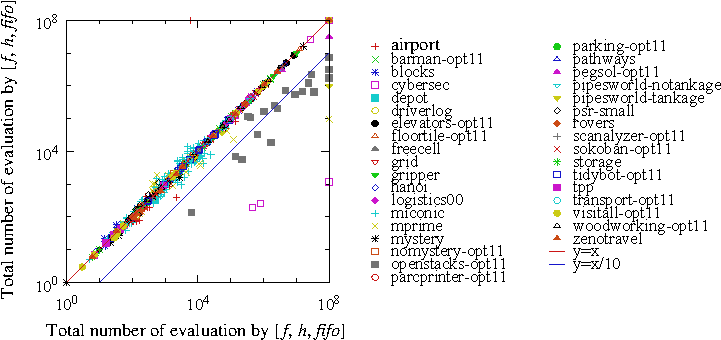
\includegraphics{tables/aaai16-30min-5min-cut/aaai16prelim3/evaluated-lmcut_ff-lmcut_lf.pdf}
 \caption{The number of LMcut evaluations on various planning domains,
 with standard \fifo vs \lifo last-resort tiebreaking, both with $h$
 tiebreaking. \lifo evaluates  less than $1/10$ of the nodes evaluated
 by \fifo in \pddl{Cybersec} and \pddl{Openstacks}. 
 }
 \label{fig:f-h-eval}
\end{figure}

% In a plateau, the heuristics do not provide any useful guidance -- a
% plateau region requires a blind search because all neighboring nodes have the same
% estimates. Because of this, search algorithms rely solely on the tiebreaking criterion.

% We further investigate the cause of this performance difference in detail.

A natural but false assumption behind this conventional wisdom would be as follows.
% 
First, the effect of the last-resort tiebreaking strategies (\lifo or
\fifo) under the presence of $h$-tiebreaking is
limited to the search plateau $\plateau{f,h}$, the set of nodes which
share the same $f$ values and $h$ values.
% 
Also, in optimal search, the two \astar with
different last-resort tiebreaking strategies both search the same set of
nodes in the region where $f<f^*$.
% 
% If $h$-tiebreaking is enabled, the two \astar variants also expands the same number of nodes with $h>0$.
Furthermore, the nodes with $h>0$ never become the goal nodes when $h$ is admissible.
% 
Therefore, the effect of last-resort tiebreaking is limited to
the final plateau $\plateau{f^*,0}$.
% 
With all these constraints, the region should sound very small compared to the
total size of the search space required to be expanded by \astar.

However, counter-intuitively, such a region can be so large enough to
cause a performance difference, or it can even account for \emph{most} of the
search effort required by \astar.
\refig{fig:plateau} plots the size of this final plateau on 1104 IPC
benchmark instances.  The $y$-axis represents the number of nodes with
$f=f^*, h=0$, the final plateau, and the $x$-axis represents the total
number of nodes expanded so far. This figure suggests that, in some
domains such as \pddl{Openstacks} and \pddl{Cybersec}, the planner
spends most of the runtime searching the final plateau for a solution,
even with the help of $h$ tiebreaking.

\begin{figure}[htbp]
   \centering
  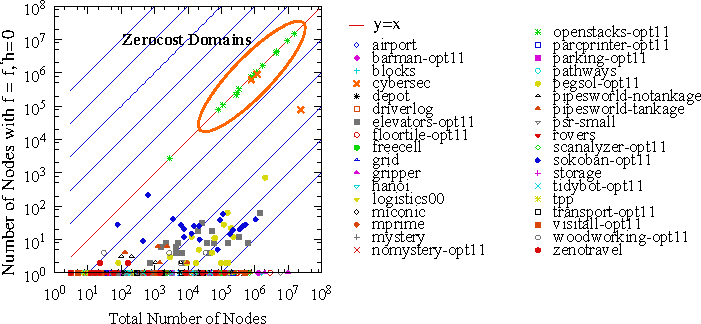
\includegraphics{tables/aaai16-frontier/aaai16prelim3/lmcut_frontier-front.pdf}
  \caption{
 The number of nodes with $f=f^*, h=0$ (y-axis), which form
  the final plateau when $h$-based tiebreaking is enabled, compared to
  the total number of nodes in the search space (x-axis) with $f\leq
  f^*$ on 1104 IPC benchmark problems.  Note that \pddl{Openstacks}
  and \pddl{Cybersec} instances are near the $y=x$ line.
  This statistics is obtained by running a modified Fast Downward with
 \lmcut which continues searching after the solution is found
 until expanding all nodes with cost $f=f^*$.} \label{fig:plateau}
\end{figure}


A natural question might be that what makes these two domains,
\pddl{Openstacks} and \pddl{Cybersec}, different from all other domains
which have much smaller final plateaus.

% \section{Domains with Zero-Cost Actions}
\label{sec:zerocost-domains}
%% best to put openstacks here, considering the connection to the
%% previous section
\pddl{Openstacks}  is a cost
minimization domain introduced in IPC-2006, where the objective is to 
minimize the number of stacks used.
There are many zero-cost actions (i.e., actions that don't increase the number of stacks), and
they prevent the standard heuristics from producing
informative guidance.

%% safe to remove these explanation.
% According to \cite{richter2010lama}, \textbf{??????}
% %Richter talks about the failures on openstacks starting around p.167
% \lmcut \cite{Helmert2009} fails to find a good cost
% partitioning with non-zero values, 
% % A detailed discussion of Openstacks domain and poor performance of landmarks is in \cite{richter10lama}, p.167-169.
% and most edges in the abstraction
% space of M\&S \cite{helmert2007flexible} have zero costs.

% XXX I'm commenting out the paragraphs below because:
% (1) A review of heuristic functions for domain-independent learning is not really
% necessary for this AAAI submission. 
% (2) It's better if this paper is not so strongly associated with the ICAPS community only -- this work applies in general to search with A*, and is not strongly tied to almost-perfect heuristics, lmcut, m&s, etc.

Although domains with zero-cost actions are not common in the current set of benchmarks, we argue that such domains are of an important class of models for cost-minimization problems, i.e.,
assigning zero costs make sense from a practical, modeling perspective.
For example, consider the \pddl{driverlog} domain, where the task is to move packages between locations using trucks.
The IPC version of this domain assigns unit costs to all actions. Thus, cost-optimal planning on this domain seeks to minimize the number of steps in the plan.
However, another natural objective function would be the one which minimizes the amount of fuel spent by driving the trucks,
assigning cost 0 to all actions except \pddl{drive-truck}.

% While I agree with the point you're trying to make,
% There is an ugly issue when arguing that current models try to  optimize plan-execution time (i.e., makespan), 
% which is that if we really cared about makespan optimality, we would consider parallel execution of actions whenever possible.
% however, sequential classical planners do not handle parallel actions at all  (recall ACP).
% so arguing this path can only lead to trouble.. Let's try a safer line of argument.
%% For runtime minimization,
%% nonzero positive costs are reasonable because
%% every actions are supposed to consume a fraction of time.
%% However, such formulation is not suitable for general optimization
%% problems.  For example, when you try to minimize the energy consumption
%% by the elevators in \pddl{Elevators} domain, many actions would have zero-cost
%% --- it does not consume electricity for either boarding or leaving the
%% passenger, or moving the elevator down.
%% % 
%% From the practical point of
%% view, cost minimization domains would have wider interest compared to
%% the simple runtime minimization.
%% Also, as shown previously, such domains pose a
%% difficulty to the current heuristic planners due to their large plateaus.

Similarly, for many practical applications, a natural objective is to
optimize the usage of one key consumable resource, e.g., fuel/energy
minimization.  In fact, two of the IPC domains, \pddl{Openstacks} and
\pddl{Cybersec}, which were shown to be difficult for standard tiebreaking
methods in the previous section, both contain many zero-cost actions,
and \textbf{both are based on industrial applications}: \pddl{Openstacks} models
production planning \cite{fink1999applications} and \pddl{Cybersec}
models Behavioral Adversary Modeling System \cite[minimizing decryption,
data transfer, etc.]{boddy2005course}.

Therefore, in this paper, we modified various domains
into cost minimization domains with many zero-cost actions.
Specifically, a domain is modified so that all action schema are assigned
cost 0 except for a few (usually one) action schema which consumes some key resource.
The last word in the names of these domains indicate the action which is
assigned non-zero cost, e.g., \pddl{elevator-up} is a modified elevator
domain where the \pddl{up} action is assigned non-zero cost (because
elevators are considered to consume energy only when going \pddl{up}), and all other actions have cost 0.
Most of the transportation-type domains are modified to optimize 
energy usage (\pddl{Logistics-fuel}, \pddl{elevator-up} etc.), and  assembly-type domains are modified to minimize resource usage
%% floortile-ink is not shown, so better not to mention it
(\pddl{Woodworking-cut} minimizes wood usage, etc.).

We did not
include domains which have only a single action schema, or which already had many zero-cost actions.
We refer to these 28 new domains as \emph{zerocost domains}.
In detail, they are:
airport-fuel (20), blocks-stack (20), depot-fuel (22), driverlog-fuel (20),
elevators-up (20), floortile-ink (20), freecell-move (20), grid-fuel (5),
gripper-move (20), hiking-fuel (20), logistics00-fuel (28), miconic-up (30),
mprime-succumb (35), mystery-feast (20), nomystery-fuel (20),
parking-movecc (20), pathways-fuel (30), pipesnt-pushstart (20),
pipesworld-pushend (20), psr-small-open (20), rovers-fuel (40),
scanalyzer-analyze (20), sokoban-pushgoal (20), storage-lift (20),
tidybot-motion (20), tpp-fuel (30), woodworking-cut (20),
zenotravel-fuel (20).

The number of instances may be different between the original domain and
the zerocost domain. One such example is \pddl{miconic}, which
originally have 150 instances while our zerocost version have
30 instances.
This is in order to reduce the effect of the difference in the
number of instances in each domain to the overall coverage sum.
In those cases, we sampled the instances evenly from the original set
of instances. For example, we picked p05, p10, ... p150 to select 30
instances.

\subsection{Difference in Problem Characteristics between IPC and Zerocost Domains}

We first tested if these new domains actually poses a new type of challenge to the
standard tiebreaking strategies. Results using \lmcut and \mands
heuristics are shown in \reftbl{tbl:lmcut-zerocost-std} and
\reftbl{tbl:mands-zerocost-std}, respectively. In each table, the left
hand side shows the results in the original domains, and the left hand side
shows the zerocost versions of the domains modified from the same
instances in the right hand side. We did not include the domains whose
number of instances differ from each other.

In both \lmcut and \mands heuristics, we observed a significant
performance difference between the original IPC domains and the zerocost
domains. With \lmcut, the coverage in zerocost domains
was lower in 11 domains, while more instances were solved
in 5 domains. With \mands, the coverage in zerocost domains was lower in 10 domains, while
more instances were solved in 3 domains.

Also, \refig{fig:plateau-zerocost} plots the size of the final plateau of the
zerocost domain instances, with \lmcut heuristics and $h$-tiebreaking. In this plot,
each point shows the total number of nodes in $\plateau{f^*,0}$ vs the
total number of nodes with $f\leq f^*$. Compared to \refig{fig:plateau},
most zerocost domains have larger plateaus even with the help of
$h$-tiebreaking.  Thus, in these cost-minimization problems, the search
strategy within plateaus, i.e., tiebreaking, becomes a yet more critical
factor which determines the search performance.

\begin{table}[htbp]
 \centering
 \setlength{\tabcolsep}{0.2em}
\begin{center}
\begin{tabular}{|lc|ccr|}
 & solved & solved & (difference) & \\
depot(22) & 6 & 6 &  & depot-fuel(22)\\
driverlog(20) & 13 & 8 & (-5) & driverlog-fuel(20)\\
elevators-opt11(20) & 15 & 7 & (-8) & elevators-up(20)\\
floortile-opt11(20) & 6 & 8 & (+2) & floortile-ink(20)\\
grid(5) & 1 & 1 &  & grid-fuel(5)\\
gripper(20) & 6 & 7 & (+1) & gripper-move(20)\\
logistics00(28) & 20 & 16 & (-4) & logistics00-fuel(28)\\
mprime(35) & 21 & 15 & (-6) & mprime-succumb(35)\\
nomystery-opt11(20) & 14 & 10 & (-4) & nomystery-fuel(20)\\
parking-opt11(20) & 1 & 0 & (-1) & parking-movecc(20)\\
pathways(30) & 5 & 5 &  & pathways-fuel(30)\\
rovers(40) & 7 & 8 & (+1) & rovers-fuel(40)\\
scanalyzer-opt11(20) & 10 & 9 & (-1) & scanalyzer-analyze(20)\\
sokoban-opt11(20) & 19 & 18 & (-1) & sokoban-pushgoal(20)\\
storage(30) & 14 & 4 & (-10) & storage-lift(20)\\
tidybot-opt11(20) & 12 & 16 & (+4) & tidybot-motion(20)\\
tpp(30) & 6 & 8 & (+2) & tpp-fuel(30)\\
woodworking-opt11(20) & 10 & 5 & (-5) & woodworking-cut(20)\\
zenotravel(20) & 11 & 7 & (-4) & zenotravel-fuel(20)\\
\end{tabular}
\end{center}

 \caption{
 Coverage comparison (the number of instances solved) 
 between the original instances and the modified zerocost instances,
 using the same configuration and experimental setting (5min, 4GB, \lmcut heuristics).
 This table does not include domains where the total number of instances
 differ in the zerocost domain and the original domain. The results in
 those domains are available in the later sections.
 }
 \label{tbl:lmcut-zerocost-std}
\end{table}

\begin{table}[htbp]
 \centering
 \begin{center}
\begin{tabular}{|lc|cr|}
 & \([f,h,\fifo]\) & \([f,h,\fifo]\) & \\
depot(22) & 6 & 5 & depot-fuel(22)\\
driverlog(20) & 12 & 9 & driverlog-fuel(20)\\
elevators-opt11(20) & 13 & 8 & elevators-up(20)\\
floortile-opt11(20) & 6 & 8 & floortile-ink(20)\\
grid(5) & 2 & 2 & grid-fuel(5)\\
gripper(20) & 20 & 20 & gripper-move(20)\\
logistics00(28) & 20 & 16 & logistics00-fuel(28)\\
mprime(35) & 23 & 21 & mprime-succumb(35)\\
nomystery-opt11(20) & 18 & 16 & nomystery-fuel(20)\\
parking-opt11(20) & 1 & 0 & parking-movecc(20)\\
pathways(30) & 4 & 4 & pathways-fuel(30)\\
rovers(40) & 8 & 8 & rovers-fuel(40)\\
scanalyzer-opt11(20) & 10 & 11 & scanalyzer-analyze(20)\\
sokoban-opt11(20) & 20 & 19 & sokoban-pushgoal(20)\\
storage(30) & 15 & 4 & storage-lift(20)\\
tidybot-opt11(20) & 0 & 0 & tidybot-motion(20)\\
tpp(30) & 7 & 9 & tpp-fuel(30)\\
woodworking-opt11(20) & 7 & 7 & woodworking-cut(20)\\
zenotravel(20) & 12 & 10 & zenotravel-fuel(20)\\
\end{tabular}
\end{center}

 \caption{
 Coverage comparison (the number of instances solved) 
 between the original instances and the modified zerocost instances,
 using the same configuration and experimental setting (5min, 4GB, \mands heuristics).
 This table does not include domains where the total number of instances
 differ in the zerocost domain and the original domain. The results in
 those domains are available in the later sections.
 }
 \label{tbl:mands-zerocost-std}
\end{table}

\begin{figure}[htbp]
  \centering
  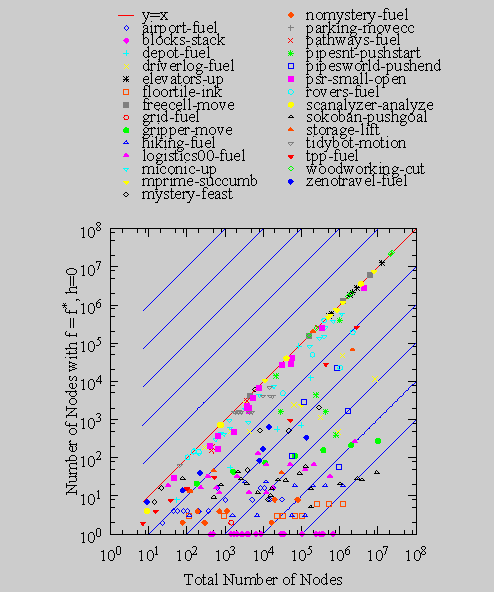
\includegraphics{tables/aaai16-frontier/zerocost/lmcut_frontier-front.pdf}
  \caption{
 The number of nodes with $f=f^*, h=0$ (y-axis), which form
  the final plateau when $h$-based tiebreaking is enabled, compared to
 the total number of nodes in the search space (x-axis) with
 $f\leq f^*$ on 620 instances in our \emph{zerocost domains}.
 The size of final plateaus tends to account for larger portion of the
 entire search space compared to \refig{fig:plateau}.
 This statistics is obtained by running a modified Fast Downward with
 \lmcut which continues searching after the solution is found
 until expanding all nodes with cost $f=f^*$.
 }
 \label{fig:plateau-zerocost}
\end{figure}

\subsection{Discussion on Zerocost Domains}

Note that the difficulty posed by these domains sometimes \emph{cannot}
be tackled by improving the heuristic estimates, or reducing the
underestimation of an admissible heuristic function.  Due to the
existence of 0-cost edges, some non-goal neighbors of a goal node can
legitimately have $h^*=0$. For those nodes,
there are no room for improving the heuristic estimate; Any positive
value causes the heuristics to be inadmissible.

There are two options to improve the search performance in such plateaus
produced by zerocost problems. The first option is to enhance the search
by combining multiple heuristics; It allows the heuristics to be
inadmissible when it is only used for tiebreaking strategy. The obvious
drawback of this strategy is the cost of additional heuristic
computation.

Another option is to perform an efficient
\emph{knowledge-free} search within plateau; It may reuse the effort
that are already spent to guide the search, but does not require
additional effort to compute multiple heuristics.
% Thus, in order to solve zerocost problems more efficiently, the planner
% needs to perform an efficient \emph{knowledge-free} search within a
% large, final plateau. 

In the next section, we first propose and evaluate an implementation of
the second option.  It turns out that a notion of \emph{depth} can have
a significant impact on the performance of knowledge-free search, as
well as a good understanding of the existing tiebreaking strategies.



% \section{Depth-Based Tiebreaking for A*}

\label{sec:depth}

As shown in the previous section, the search spaces of Zerocost domains have many zero-cost edges,
resulting in a large final plateau ($\plateau{f^*,0}$). In a final plateau,
all nodes have $h=0$, so $h$-based tiebreaking cannot provide
useful guidance toward a goal. Thus, we need a new metric for discriminating among nodes
in the plateau so that the search algorithm can make progress in the plateau.

We define the \emph{depth} of a node as an 
integer representing the distance (number of steps) from the
\emph{entrance} of the plateau.  An \emph{entrance} of the plateau is
the first node which encountered in the plateau, along the path from the
initial node. These notions are depicted in
\refig{fig:plateau-depiction} (subfigure 1). 
Another way to think about depth is consider the problem of finding an exit from a particular plateau (i.e., finding either a goal node or exhausting the plateau) a unit-cost search space by itself -- the depth is analogous to a $g$-value for this space.
%It is equivalent to the $g$-value which is
%restricted to a particular plateau and is assuming the unit cost edges.

\begin{figure}[htbp]
  \centering
  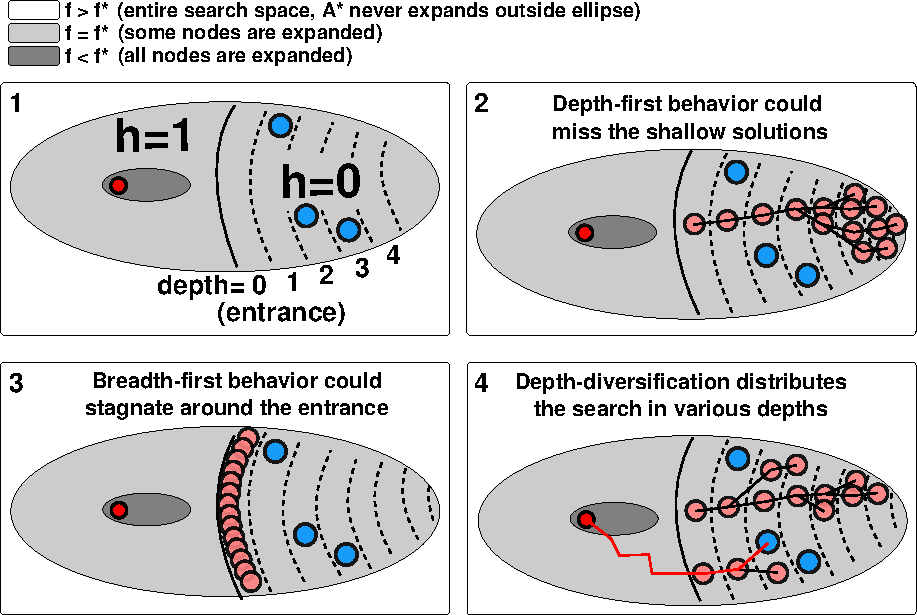
\includegraphics{img/astar/plateau-2.pdf}
 \caption{(\textbf{Subfigure 1}) The nodes in a plateau are divided into several layers, and each layer have the corresponding depth. Since all nodes have $f=f^*$, depth does not affect optimality. The goals in both shallower or deeper region yield cost-optimal solutions.
 (\textbf{Subfigure 2}) \lifo tiebreaking strategy results in depth-first behavior in a
 plateau, which could miss solutions if they are concentrated near the entrance.
 (\textbf{Subfigure 3}) \fifo tiebreaking strategy results in  breadth-first behavior in a
 plateau, which could fail to reach a solutions in deeper layers within the time limit.
 (\textbf{Subfigure 4}) Depth-based diversification allows \astar to search the plateau space
 sparsely in a less biased, more uniformly and manner. This balances exploration and exploitation, avoiding the problems with both \lifo (depth-first) and \fifo (breadth-first) behavior.
 }
 \label{fig:plateau-depiction}
\end{figure}

The depth $d(n)$ of a
node $n$ is 0 when $n$ and the parent node $m$ have different key
values for a sorting strategy, and $d(n)=d(m)+1$ when they have the same
key values: For example, in \astar with $h$-based tiebreaking, the key
values of a node are represented as a vector $[f,h]$, and they are same
when they are pairwise equivalent (i.e. $f(n) = f(m) \land h(n) =
h(m)$).  Having the same key values means that $n$ and $m$ are in the
same plateau.

The traditional \lifo and \fifo tiebreaking strategy 
search the plateau region in decreasing and increasing order of the depth, respectively.
The \lifo strategy always selects the most recently generated node
within $\plateau{f,h}$, and the behavior in the plateau is equivalent to depth-first search.
Thus, \lifo always selects the largest depth
buckets, as depicted in \refig{fig:plateau-depiction} (subfigure 2).
Similarly, the behavior of the \fifo strategy 
in a plateau is equivalent to breadth-first search. Thus \fifo 
always selects the nodes with least depth (subfigure 3).
Note that  $[f,h,\lifo]$ is equivalent to $[f,h,-d,\lifo]$ and
$[f,h,\fifo]$ is equivalent to $[f,h,d,\fifo]$.

The problem with these traditional strategies is that we have no knowledge
regarding whether the goals are located close to or far from the entrance. Recall
that since $f=f^*$, all goal nodes in the final plateau are optimal with respect to solution cost.
regardless of the depth.%: A goal node in a shallower region or a deeper region both yields a cost-optimal solution. 
However, until we find a
solution, we do not know how the goals are distributed among various
depths. In some problem instance the goals can be concentrated around
the entrance, and in other problem instances the goals can be
concentrated at some large depth. % $k$.  k never used below?

In the former case, (\fifo), whose breadth-first behavior naturally
focuses the search around the entrance favoring the smaller depths,
should perform well, but in the latter case, exhaustively searching
the shallower depths can result in not finding any solutions within
the time limit because \fifo may never reach the depth where the goals
exist.  On the other hand, \lifo behaves in a depth-fist manner, so it
may reach solutions at deeper depths quickly, but risks missing
solutions at shallower depths.  Thus, both \fifo and \lifo tiebreaking
are prone to failures due to pathological cases.

In order to avoid focusing the search at the wrong depths (too shallow/deep), 
the safest policy seems to be to simply \emph{diversify} the depths which are being searched,
in order to avoid any depth-based biases which could lead to pathological behavior.
In our proposed \emph{depth diversification} strategy, the nodes are inserted into buckets
associated with depths, and upon expansion, search effort is distributed in a more balanced manner
among various depths (\refsec{sec:theoretical-characteristics} defines ``more balanced''  more precisely).
Nodes are not  ``sorted''
according to increasing or decreasing order of depth -- instead we try to 
``diversify'' the node expansion within the plateau.
We denote this depth diversification criterion as $\depth$. 
For example, $[f,h,\depth]$ first breaks ties according to $h$ values,
then uses the $\depth$ criterion to break ties in $\plateau{f,h}$.
%We denote such a diversification family of
%tiebreaking strategies by enclosing it in brackets such as $[f,h,\depth]$.

In order to diversify the expansion among depths, we simply
iterate over the depth buckets. An index $d_c$,
 which stores the depth (bucket index)  which was selected in the last expansion,
is initialized to 0.
At each expansion, the counter is decremented ($d_c\leftarrow d_c-1$) and
a node from  bucket $d_c$ is expanded. When $d_c$ reaches below 0, then $d_c$
is reset to the current largest depth in the plateau.

In an earlier, conference paper, we used a non-deterministic,
randomized implementation of this idea \cite{Asai16}, but we use a deterministic
implementation here because it eliminates the possibility of results being influenced by random seeds,
and also facilitates the  theoretical analysis below in \refsec{sec:theoretical-characteristics}.

% We later show that
% \fifo and \lifo strategies are incomplete when the size of the plateau
% region is inifinite, while our \id is probabilistically complete.

\subsection{The Scope Captured by Depth-Based Tiebreaking}

Depth-based tiebreaking has no effect when the key values for measuring
the depth are always updated and thus all nodes have depth 0. A key
value is a single $f$ when $h$-based tiebreaking is not present, and a
pair of $f$ and $h$ when $h$-based tiebreaking is present. When all
nodes have depth 0, the search is equivalent to the case where 
the depth-based strategy is not present.\todo{mentioning ``keys'' seems unnecessarily complicated, and  ```key'' doesn't seem to be used much in the rest of the paper -- simpler+sufficient to just say that 
``depth diversification has no effect when there are no plateaus after the higher priority tiebreaking criteria (e.g., in a [f,h,<d>] strategy, when there are no [f,h] plateaus), which occurs when the problem only has positive cost operators'' ?}
% 
This happens when the target problem only has 
operators with positive cost. %\footnote{not to be confused with non-negative cost.  XXXshouldn't be necessary, positive doesn't include 0 for any standard def} 
Let a node $n$ is reached from a node $m$. \todo{is this par necessary?}
Assume
 $g(n)>g(m)+c$ where $c$ is a positive edge cost, and the parent of $n$
 is updated to $m$.

\begin{itemize}
 \item 
       If $f(n)=f(m)$, $h(n)<h(m)$ should hold because the new value of
       $g(n)$ is $g(m)+c>g(m)$. Therefore the depth is 0.
 \item If $h$-value is unchanged and $g$ is increased due to a positive
       cost edge, then $f$ is also increased, thus the depth is 0.
\end{itemize}

One might wonder what if the evaluated (?) nodes (?) are already visited (?) from
another parent (old (?)parent) with smaller $g$ value, and the new $g$ value does not change it (?),
which may cause the new parent and the child node may have the same $f$ and
same $h$. It does not result in a positive depth because it does not update the parent. The depth of a
child remains the old value (using the old parent), which is 0.\todo{rewrite par -- terminology is inconsistent and pronouns are ambiguous}


\subsection{Tiebreaking within Depth Buckets}

Consider a tiebreaking strategy such as $[f,h,\depth]$ which applies a depth-diversification tiebreaking.
After the $\depth$ criterion is applied, 
there may be multiple nodes within the same depth bucket, so a
default tiebreaking criterion is still necessary to break ties among them.
We can, for example, apply \lifo, \fifo or \ro (random order) policies
at this level.

There could be still a room for heuristic-agnostic improvements at
this level, \todo{what is ``this level'': same level as $\depth$ (in which case these 2 pars don't seem to fit in this subsection), or after depth?} while this is not in the scope of this paper.
For example, while depth metric measures and diversifies the depth in a plateau,
other techniques can non-trivially diversify the search in a breadth direction.
Such techniques may include pruning techniques such as 
Symmetry Breaking \cite{Fox1998,pochter2011exploiting,domshlak2013symmetry}
or Partial Order Reduction \cite{hall2013faster,wehrle2013relative}.

While these methods are most often described as ``pruning techniques'',
it can be rephrased as ``removing the cardinality bias to particular set
of nodes which share the same characteristics'' because they both aim to
prune the redundant nodes. Note that redundancy causes a biased 
search effort. For example, imagine we have a
set of nodes $S=\{a_1, a_2, a_3, a_4, b, c, d\}$ where
$A=\{a_1, a_2, a_3, a_4\}$ are ``redundant'' in some measure (e.g. by Symmetry,
Partial-Order). 
If a search algorithm expands $S$ by random selection, it favors the
group $A$ by giving a 4 times larger chance of expansion than $b$,
$c$ or $d$.

% \todo{compare id,fifo and id,lifo}
CommentOnTheDeletedActionOrderingText\todo{Although there's no need to show new results for action ordering, 
it may be a good idea to summarize+point to the AAAI16 action ordering experiment, in order to eliminate concerns that
all our results are somehow specific to one particular action order.}
% However we use a Random Order (\ro) criterion, which 
% randomly selects an element from the depth bucket selected by the depth-based tiebreaking.
% This is because the effectiveness of the tiebreaking behavior within a bucket
% can be affected by accidental biases, e.g., names/orders of action schema in the PDDL domain
% definition \cite{vallati2015effective}.
% %Finding the best action ordering is not the scope of this paper.
% Thus, we avoid bias at this level of tiebreaking by using \ro and assess its expected/average
% performance.

% Among \fifo, \lifo and \ro, the natural criterion is Random Order.
% This is because the effectiveness of the third-level tiebreaking behavior
% is affected by the accidental bias in action ordering in the PDDL domain
% definition.  Recent work \cite{vallati2015effective} showed that the
% planner performance is greatly affected by changing and tuning the action ordering
% (and also variable ordering, but it is irrelevant to the tiebreaking behavior). 
% However, finding the best third-level tiebreaking is not the scope of this paper.
% Thus, focusing on \ro and assess its expected/average
% performance is the most reasonable practice to understand the behavior of second-level,
% depth-based tiebreaking.

\subsection{Theoretical Characteristics of the Depth Distribution}
\label{sec:theoretical-characteristics}

We give further insight into the search behavior of our implementation
of depth-based diversification.
As described above, our implementation performs a deterministic, round-robin sampling from the available depth buckets.
%iterates from the largest depth to 0.

%We are particularly interested in how the expansions happen among the
%various depths in the plateau region.
We are particularly interested in how the nodes selected for expansion are distributed 
among the various depths in a plateau region.
Using a simplified model where the plateau region is a tree,
we show that the probability of expanding a node in a particular depth
can be represented by a simple formula.  Although the notion of
probability does not fit well with deterministic \fifo or \lifo
default tiebreaking, it is meaningful in the case of \ro (random
order) default tiebreaking.

%% danger!!
% \begin{theo}[Uniformness of the search]
%  Assume the search space forms a tree of fixed width $w\geq 2$.
%  After enough number of iterations $D$,
%  the chance of expanding each node is unaffected by the depth of the
%  node, if the depth $d$ is small relative to $D$.
% \end{theo}

% I no longer claim the distribution is uniform.
As a preparation, we first show that the number of expansion happened to each depth decreases
linearly to the depth.
% 
\todo*{Introduced the tree assumption in the beginning.}
We first assume that the plateau region form a tree of a fixed branching factor
$w\geq 2$ (\emph{tree assumption}), rather than a graph with indefinite number of successor nodes.
We also assume that no depth buckets exhaust due to the expansion (\emph{no-exhaust assumption}).

Let $D\geq 0$ be the current largest depth of the nodes found in the plateau so far.  If the expansion of a node in
depth $D$ resulted in more nodes in the same plateau, then the children have depth $D+1$.  Due to the tree
assumption, these children are all newly generated. Also, as we explained in the previous section, the expansion is
diversified by a sequence of iterations from the current largest depth to 0.  It means that when the current
largest depth of the plateau is $D$, the number of iteration happened so far is also $D$.
% Under the tree assumption, each expansion of depth $d$ results in $w$ new nodes in depth $d+1$. 
Therefore, at the end of the $D$'th iteration, each depth $d$ has been expanded exactly $D-d$ times, with $D(D-1)$
expansions in total.

It also means that the minimum condition for \emph{no-exhaust assumption} to hold until the end of the $D$'th
iteration is that the initial number of nodes in depth 0 is at least $D$.  If there are at least $D$ nodes in depth
0, depth 0 trivially never exhausts until $D$'th iteration. Also, no depth buckets in depth $d>0$ will exhaust
because each bucket have $w^{D-d-1}$ nodes in total (including those already expanded) while the expansion has
happened only $D-d$ times. For simplicity, let us also assume that the depth 0 initially have exactly $D$ nodes and
no nodes will be added to depth 0 during the search.

Now we show the formula which represents the probability of expanding a node in a particular depth.
At the end of $D$'th iteration,
each depth $d-1$ is expanded $D-(d-1)$ times in the preceding $D$ iterations.
Therefore, the total number of nodes that have been in depth $d$, including those
that have been expanded so far, is $w(D-d+1)$.
Expansion has happened $D(D-1)$ times in total, and depth $d$ is expanded $D-d$ times.
Thus, the probability of expanding each node in depth $d$ is
$\frac{D-d}{D(D-1)\cdot w(D-d+1)}=\frac{1}{wD(D-1)}(1-\frac{1}{D-d+1})$.  \qed

Notice that $\frac{1}{D-d+1}$ is negligible if $D \gg d$.
Thus, after enough number of iterations (large $D$), the nodes are 
expanded in an approximately equal probability $\frac{1}{wD(D-1)}$ in the shallower region, and is
unaffected by the depth of the node.
However, the nodes near the largest depth has less probability, showing
some balance in exploration and exploitation.

The important point of this characteristics is that this distribution is maintained at any point of the search
until the solution is found. In fact, any depth-selection criterion, including the least depth selection (\fifo) or
the largest depth selection (\lifo), result in the same distribution if all nodes are to be expanded (each depth
$d$ is expanded $Dw^d$ times), but their online characteristics are not.
%
\todo*{maybe \lifo and \fifo should be analyzed wrto this tree model and compared directly to each other as well as
$\depth$?}
\todo*{less priority -- lets add it when required by the reviewers. unused texts are in unused/lifo-fifo-distribution.tex}



\section{Evaluating Depth-Based Tiebreaking}
\label{sec:depth-based-evaluation}
We evaluated our depth-based diversifying tiebreaking strategies against standard
tiebreaking strategies.
In addition to the 35 IPC benchmark domains with 1104 instances used in
the previous set of experiments, we used 28 zerocost domains with 620
instances.

\subsection{Evaluating Depth-Based Tiebreaking with $h$-tiebreaking}

We compared the performance of standard tiebreaking methods $[f,h,\fifo]$,
$[f,h,\lifo]$ to $[f,h,\brackets{d},\fifo]$ and
$[f,h,\brackets{d},\lifo]$.  These all use $h$ as the first-level
tiebreaking and either \fifo or \lifo as the last-resort tiebreaking.

First two experiments are conducted on \textbf{1104 standard IPC
benchmark instances}, and the latter two experiments are conducted on
\textbf{620 zerocost instances}.  Each experiment uses either \lmcut
heuristics or \mands heuristics.  For \mands heuristics, we used the
settings recommended by Fast Downward website (bisimulation-based shrink
strategy, DFP merge strategy and exact label reduction).

We first show the summary results of these experiments.
Overall, depth-based tiebreaking tends to show larger coverages than the
standard tiebreaking strategies. In the following, we describe the
details of each experiments.

\begin{table}[htb]
 {
 \centering
\begin{tabular}{|*{5}{c|}}
\hline
 & \multicolumn{4}{|c|}{\lmcut Coverages (\# problems solved)}\\
\hline                                    
 Domain               &  $[f,h,\fifo]$ &  $[f,h,\lifo]$ &  $[f,h,\brackets{d},\fifo]$ &  $[f,h,\brackets{d},\lifo]$ \\ \hline
 IPC,\lmcut(1104)     &558             &565             &\textbf{570.6\spm{}1.5}      &560.0\spm{}0.9               \\ 
 IPC,\mands(1104)     &479             &\textbf{488}    &484.0\spm{}0.0               &481.4\spm{}1.4               \\ \hline
 Zerocost,\lmcut(620) &256             &279             &\textbf{287.2\spm{}2.4}      &280.2\spm{}4.2               \\ 
 Zerocost,\mands(620) &276             &290             &\textbf{310.2\spm{}2.1}      &303.2\spm{}1.7               \\ \hline
\end{tabular}
 \caption{
 Summary Results: Coverage comparison (the number of instances solved in 5min, 2GB, \lmcut/\mands
 heuristics) between standard tiebreaking and depth-based tiebreaking ($\brackets{d}$). }
 \label{tbl:lmcut-ipc-full}
 }
\end{table}

\reftbl{tbl:lmcut-ipc-full} shows the number of \textbf{1104 standard
IPC benchmark instances} solved by \lmcut heuristics with various
tiebreaking strategies, under 5min, 2GB experiments. We highlight the
best results when the difference between the maximum and the mininum
coverage exceeds 2.  Depth-based tiebreaking ($\brackets{d}$) shows
impressive results on Openstacks and Cybersec domains because these
domains contain many instances of zero-cost edges and the final plateau
$\plateau{f,h}$ is huge (See \refig{fig:plateau}).  Most other instances
are unaffected by depth-based tiebreaking.  Thus, our method offers a
better performance in the domains of interest for free, i.e. without
losing performance in other domains.

\begin{table}[htbp]
 {
 \centering
 \begin{tabular}{|*{5}{c|}}
\hline
 & \multicolumn{4}{|c|}{\lmcut Coverages (\# problems solved)}\\
\hline                                    
 Domain                                 &  $[f,h,\fifo]$ &  $[f,h,\lifo]$ &  $[f,h,\brackets{d},\fifo]$       &  $[f,h,\brackets{d},\lifo]$        \\ \hline                                    
 sum(1104)                              &558             &565             &\textbf{570.6\spm{}1.5} &560.0\spm{}0.9         \\ \hline                                    
 {\relsize{-1}airport(50)}              &\textbf{27}     &26              &25.9\spm{}0.5           &21.0\spm{}0.0          \\
 {\relsize{-1}barman-opt11(20)}         &0               &0               &0.0\spm{}0.0            &0.0\spm{}0.0           \\
 {\relsize{-1}blocks(35)}               &28              &28              &28.0\spm{}0.0           &27.0\spm{}0.0          \\
 {\relsize{-1}cybersec(19)}             &2               &3               &\textbf{9.6\spm{}1.1}   &7.8\spm{}0.7           \\
 {\relsize{-1}depot(22)}                &6               &6               &6.0\spm{}0.0            &6.0\spm{}0.0           \\
 {\relsize{-1}driverlog(20)}            &13              &13              &13.0\spm{}0.0           &13.0\spm{}0.0          \\
 {\relsize{-1}elevators-opt11(20)}      &15              &15              &15.0\spm{}0.0           &14.8\spm{}0.4          \\
 {\relsize{-1}floortile-opt11(20)}      &6               &6               &6.0\spm{}0.0            &6.0\spm{}0.0           \\
 {\relsize{-1}freecell(80)}             &9               &9               &9.0\spm{}0.0            &9.0\spm{}0.0           \\
 {\relsize{-1}grid(5)}                  &1               &1               &1.0\spm{}0.0            &1.0\spm{}0.0           \\
 {\relsize{-1}gripper(20)}              &6               &6               &6.0\spm{}0.0            &6.0\spm{}0.0           \\
 {\relsize{-1}hanoi(30)}                &12              &12              &12.0\spm{}0.0           &12.0\spm{}0.0          \\
 {\relsize{-1}logistics00(28)}          &\textbf{20}     &\textbf{20}     &\textbf{20.0\spm{}0.0}  &\textbf{20.0\spm{}0.0} \\
 {\relsize{-1}miconic(150)}             &\textbf{140}    &\textbf{140}    &\textbf{140.0\spm{}0.0} &135.6\spm{}0.5         \\
 {\relsize{-1}mprime(35)}               &21              &21              &20.9\spm{}0.3           &21.0\spm{}0.0          \\
 {\relsize{-1}mystery(30)}              &15              &16              &15.0\spm{}0.0           &15.8\spm{}0.4          \\
 {\relsize{-1}nomystery-opt11(20)}      &14              &14              &14.0\spm{}0.0           &13.8\spm{}0.4          \\
 {\relsize{-1}openstacks-opt11(20)}     &11              &\textbf{18}     &\textbf{18.0\spm{}0.0}  &\textbf{18.0\spm{}0.0} \\
 {\relsize{-1}parcprinter-opt11(20)}    &13              &13              &13.0\spm{}0.0           &13.0\spm{}0.0          \\
 {\relsize{-1}parking-opt11(20)}        &1               &1               &1.0\spm{}0.0            &1.0\spm{}0.0           \\
 {\relsize{-1}pathways(30)}             &5               &5               &5.0\spm{}0.0            &5.0\spm{}0.0           \\
 {\relsize{-1}pegsol-opt11(20)}         &17              &17              &17.0\spm{}0.0           &17.0\spm{}0.0          \\
 {\relsize{-1}pipesworld-notankage(50)} &15              &14              &14.2\spm{}0.4           &14.2\spm{}0.4          \\
 {\relsize{-1}pipesworld-tankage(50)}   &8               &8               &8.0\spm{}0.0            &8.0\spm{}0.0           \\
 {\relsize{-1}psr-small(50)}            &48              &48              &48.0\spm{}0.0           &48.0\spm{}0.0          \\
 {\relsize{-1}rovers(40)}               &7               &7               &7.0\spm{}0.0            &7.0\spm{}0.0           \\
 {\relsize{-1}scanalyzer-opt11(20)}     &\textbf{10}     &\textbf{10}     &\textbf{10.0\spm{}0.0}  &9.0\spm{}0.0           \\
 {\relsize{-1}sokoban-opt11(20)}        &19              &19              &19.0\spm{}0.0           &19.0\spm{}0.0          \\
 {\relsize{-1}storage(30)}              &14              &14              &14.0\spm{}0.0           &14.4\spm{}0.5          \\
 {\relsize{-1}tidybot-opt11(20)}        &12              &12              &12.0\spm{}0.0           &11.8\spm{}0.4          \\
 {\relsize{-1}tpp(30)}                  &6               &6               &6.0\spm{}0.0            &6.0\spm{}0.0           \\
 {\relsize{-1}transport-opt11(20)}      &6               &6               &6.0\spm{}0.0            &6.0\spm{}0.0           \\
 {\relsize{-1}visitall-opt11(20)}       &10              &10              &10.0\spm{}0.0           &10.0\spm{}0.0          \\
 {\relsize{-1}woodworking-opt11(20)}    &10              &10              &10.0\spm{}0.0           &\textbf{11.8\spm{}0.4} \\
 {\relsize{-1}zenotravel(20)}           &11              &11              &11.0\spm{}0.0           &11.0\spm{}0.0          \\\hline
\end{tabular}

 \caption{
 Coverage comparison (the number of instances solved in 5min, 2GB, LMcut
 heuristics) on \textbf{1104 standard IPC benchmark instances}. We highlight the
 best results when the difference between the maximum and the mininum coverage exceeds 2.
 }
 \label{tbl:lmcut-ipc-full}
 }
\end{table}


\reftbl{tbl:mands-ipc-full} shows the results by \mands heuristics.
In this configuration, depth-based tiebreaking negatively affects the performance.
As we show in \reftbl{tbl:expansion-ratio}, this is because
the low-level overhead of depth-based tiebreaking decreases the high
node processing speed of \mands. Evaluation of \mands heuristics is
very efficiently implemented as a table lookup, and it is able to
evaluate an order of magnutude larger number of nodes
compared to \lmcut heuristics.

\reftbl{tbl:mands-evaluations} shows that if we instead compare the
number of evaluations on problems solved by both, depth-based
tiebreaking significantly outperforms the standard tiebreaking
strategies. Moreover, in the next \textbf{zerocost} domain experiments,
depth-based tiebreaking ourperforms the standard tiebreaking
overall. Besides, the coverages by \mands is less than that of \lmcut.

\begin{table}[htbp]
 {
 \centering
 \begin{tabular}{|*{5}{c|}}
\hline
 & \multicolumn{4}{|c|}{\mands Coverages (\# problems solved)}\\
\hline                                    
 Domain                                 &  $[f,h,\fifo]$ &  $[f,h,\lifo]$ &  $[f,h,\brackets{d},\fifo]$       &  $[f,h,\brackets{d},\lifo]$        \\ \hline                                    
 sum(1104)                              &479             &\textbf{488}    &484.0\spm{}0.0         &481.4\spm{}1.4          \\ \hline
 {\relsize{-1}airport(50)}              &9               &9               &9.0\spm{}0.0           &9.0\spm{}0.0            \\
 {\relsize{-1}barman-opt11(20)}         &4               &4               &4.0\spm{}0.0           &4.0\spm{}0.0            \\
 {\relsize{-1}blocks(35)}               &22              &21              &21.6\spm{}0.5          &21.8\spm{}0.4           \\
 {\relsize{-1}cybersec(19)}             &0               &0               &0.0\spm{}0.0           &0.0\spm{}0.0            \\
 {\relsize{-1}depot(22)}                &5               &6               &5.0\spm{}0.0           &5.0\spm{}0.0            \\
 {\relsize{-1}driverlog(20)}            &12              &12              &12.0\spm{}0.0          &12.0\spm{}0.0           \\
 {\relsize{-1}elevators-opt11(20)}      &12              &12              &12.0\spm{}0.0          &12.0\spm{}0.0           \\
 {\relsize{-1}floortile-opt11(20)}      &6               &6               &6.0\spm{}0.0           &5.2\spm{}0.4            \\
 {\relsize{-1}freecell(80)}             &17              &17              &16.0\spm{}0.0          &15.6\spm{}0.5           \\
 {\relsize{-1}grid(5)}                  &2               &2               &2.0\spm{}0.0           &2.0\spm{}0.0            \\
 {\relsize{-1}gripper(20)}              &20              &20              &20.0\spm{}0.0          &20.0\spm{}0.0           \\
 {\relsize{-1}hanoi(30)}                &14              &14              &14.0\spm{}0.0          &14.0\spm{}0.0           \\
 {\relsize{-1}logistics00(28)}          &20              &20              &20.0\spm{}0.0          &20.0\spm{}0.0           \\
 {\relsize{-1}miconic(150)}             &\textbf{73}     &\textbf{73}     &\textbf{73.0\spm{}0.0} &72.4\spm{}0.5           \\
 {\relsize{-1}mprime(35)}               &23              &24              &23.4\spm{}0.5          &23.2\spm{}0.7           \\
 {\relsize{-1}mystery(30)}              &15              &16              &15.0\spm{}0.0          &15.0\spm{}0.0           \\
 {\relsize{-1}nomystery-opt11(20)}      &18              &18              &18.0\spm{}0.0          &18.0\spm{}0.0           \\
 {\relsize{-1}openstacks-opt11(20)}     &13              &\textbf{19}     &\textbf{19.0\spm{}0.0} &\textbf{19.0\spm{}0.0}  \\
 {\relsize{-1}parcprinter-opt11(20)}    &9               &9               &9.0\spm{}0.0           &9.0\spm{}0.0            \\
 {\relsize{-1}parking-opt11(20)}        &1               &1               &1.0\spm{}0.0           &1.0\spm{}0.0            \\
 {\relsize{-1}pathways(30)}             &4               &4               &4.0\spm{}0.0           &4.0\spm{}0.0            \\
 {\relsize{-1}pegsol-opt11(20)}         &19              &19              &19.0\spm{}0.0          &18.8\spm{}0.4           \\
 {\relsize{-1}pipesworld-notankage(50)} &8               &9               &8.0\spm{}0.0           &8.0\spm{}0.0            \\
 {\relsize{-1}pipesworld-tankage(50)}   &13              &13              &13.0\spm{}0.0          &13.0\spm{}0.0           \\
 {\relsize{-1}psr-small(50)}            &50              &50              &50.0\spm{}0.0          &50.0\spm{}0.0           \\
 {\relsize{-1}rovers(40)}               &8               &8               &8.0\spm{}0.0           &7.6\spm{}0.5            \\
 {\relsize{-1}scanalyzer-opt11(20)}     &10              &10              &10.0\spm{}0.0          &10.4\spm{}0.5           \\
 {\relsize{-1}sokoban-opt11(20)}        &19              &19              &19.0\spm{}0.0          &18.4\spm{}0.5           \\
 {\relsize{-1}storage(30)}              &15              &15              &15.0\spm{}0.0          &15.0\spm{}0.0           \\
 {\relsize{-1}tidybot-opt11(20)}        &0               &0               &0.0\spm{}0.0           &0.0\spm{}0.0            \\
 {\relsize{-1}tpp(30)}                  &6               &6               &6.0\spm{}0.0           &6.0\spm{}0.0            \\
 {\relsize{-1}transport-opt11(20)}      &6               &6               &6.0\spm{}0.0           &6.0\spm{}0.0            \\
 {\relsize{-1}visitall-opt11(20)}       &9               &9               &9.0\spm{}0.0           &9.0\spm{}0.0            \\
 {\relsize{-1}woodworking-opt11(20)}    &7               &7               &7.0\spm{}0.0           &7.0\spm{}0.0            \\
 {\relsize{-1}zenotravel(20)}           &10              &10              &10.0\spm{}0.0          &10.0\spm{}0.0           \\\hline
\end{tabular}

 \caption{
 Coverage comparison (the number of instances solved in 5min, 2GB, M\&S
 heuristics) on \textbf{1104 standard IPC benchmark instances}. We highlight the
 best results when the difference between the maximum and the mininum coverage exceeds 2.
 }
 \label{tbl:mands-ipc-full}
 }
\end{table}

\begin{table}[htb]
 \centering
 \begin{tabular}{cccc}
  nodes/sec                  & LMcut      & M\&S       & M\&S slowdown\\
  \hline
  $[f,h,\lifo]$              & 8.86$\times 10^3$ & 1.37$\times 10^5$ & 100\%\\
  $[f,h,\brackets{d},\lifo]$ & 9.37$\times 10^3$ & 1.13$\times 10^5$ & 82\%\\
  \hline
  $[f,h,\fifo]$              & 9.65$\times 10^3$ & 1.41$\times 10^5$ & 100\%\\
  $[f,h,\brackets{d},\fifo]$ & 9.62$\times 10^3$ & 1.24$\times 10^5$ & 87\%\\
  \hline
 \end{tabular}
 \caption{Comparison of the average node expansion ratio (node/sec) between
 standard tiebreaking and depth-based tiebreaking on \lmcut and \mands
 heuristics. Numbers are averaged over the problem instances solved by
 all 4 configurations. Since the node evaluation of \mands is an order of
 magnitude faster than \lmcut, the overhead of managing depth-based
 tiebreaking queue is non-negligeble on \mands.}
 \label{tbl:expansion-ratio}
\end{table}

\begin{figure}[htb]
 \centering
 \caption{Comparison of the total number of nodes generated by \mands
 heuristics, with vs without depth-based tiebreaking.}
 \label{tbl:mands-evaluations}
\end{figure}

In zerocost domains, our proposed method outperforms the traditional
tiebreaking methods in both \lmcut and \mands heuristics
(\reftbl{tbl:lmcut-zerocost-full} and \reftbl{tbl:mands-zerocost-full}).
Significant improvements were observed in X domains when using \lmcut,
and in X domains when using \mands.

\begin{table}[htbp]
 {
 \centering
 \begin{tabular}{|*{5}{c|}}
\hline
 & \multicolumn{4}{|c|}{Coverages (\# problems solved)} \\ \hline
 Domain                               &  $[h,\fifo]$ &  $[h,\lifo]$ &  $[h,\rd,\ro]$         &  $[\rd,\ro]$          \\ \hline
 sum(620)                             &256           &279           &\textbf{287.2\spm{}2.4} &280.2\spm{}4.2         \\ \hline
 {\relsize{-1}airport-fuel(20)}       &\textbf{15}   &13            &14.4\spm{}0.7           &10.4\spm{}0.5          \\
 {\relsize{-1}blocks-stack(20)}       &17            &17            &17.0\spm{}0.0           &16.0\spm{}0.0          \\
 {\relsize{-1}depot-fuel(22)}         &6             &6             &6.0\spm{}0.0            &6.0\spm{}0.0           \\
 {\relsize{-1}driverlog-fuel(20)}     &8             &8             &8.0\spm{}0.0            &8.0\spm{}0.0           \\
 {\relsize{-1}elevators-up(20)}       &7             &\textbf{13}   &9.4\spm{}1.1            &8.2\spm{}0.7           \\
 {\relsize{-1}floortile-ink(20)}      &8             &8             &8.1\spm{}0.3            &8.0\spm{}0.0           \\
 {\relsize{-1}freecell-move(20)}      &4             &19            &16.5\spm{}0.7           &16.6\spm{}0.8          \\
 {\relsize{-1}grid-fuel(5)}           &1             &1             &1.0\spm{}0.0            &1.0\spm{}0.0           \\
 {\relsize{-1}gripper-move(20)}       &7             &7             &6.0\spm{}0.0            &7.0\spm{}0.0           \\
 {\relsize{-1}hiking-fuel(20)}        &9             &9             &9.0\spm{}0.0            &9.0\spm{}0.0           \\
 {\relsize{-1}logistics00-fuel(28)}   &16            &16            &15.0\spm{}0.0           &16.0\spm{}0.0          \\
 {\relsize{-1}miconic-up(30)}         &16            &17            &\textbf{19.8\spm{}1.0}  &20.4\spm{}1.0          \\
 {\relsize{-1}mprime-succumb(35)}     &15            &14            &\textbf{20.1\spm{}0.7}  &18.6\spm{}2.0          \\
 {\relsize{-1}mystery-feast(20)}      &7             &5             &7.2\spm{}0.4            &7.2\spm{}0.7           \\
 {\relsize{-1}nomystery-fuel(20)}     &10            &10            &10.0\spm{}0.0           &9.4\spm{}0.5           \\
 {\relsize{-1}parking-movecc(20)}     &0             &0             &0.0\spm{}0.0            &0.0\spm{}0.0           \\
 {\relsize{-1}pathways-fuel(30)}      &5             &5             &4.4\spm{}0.5            &4.8\spm{}0.4           \\
 {\relsize{-1}pipesnt-pushstart(20)}  &8             &8             &\textbf{9.8\spm{}0.4}   &\textbf{9.8\spm{}0.4}  \\
 {\relsize{-1}pipesworld-pushend(20)} &3             &4             &4.5\spm{}0.8            &\textbf{5.4\spm{}0.8}  \\
 {\relsize{-1}psr-small-open(20)}     &19            &19            &19.0\spm{}0.0           &19.0\spm{}0.0          \\
 {\relsize{-1}rovers-fuel(40)}        &8             &8             &8.0\spm{}0.0            &9.0\spm{}0.0           \\
 {\relsize{-1}scanalyzer-analyze(20)} &9             &9             &9.1\spm{}0.3            &7.4\spm{}1.0           \\
 {\relsize{-1}sokoban-pushgoal(20)}   &18            &18            &17.9\spm{}0.3           &17.0\spm{}0.0          \\
 {\relsize{-1}storage-lift(20)}       &4             &4             &4.4\spm{}0.5            &4.6\spm{}0.5           \\
 {\relsize{-1}tidybot-motion(20)}     &16            &16            &16.0\spm{}0.0           &15.6\spm{}0.5          \\
 {\relsize{-1}tpp-fuel(30)}           &8             &\textbf{11}   &\textbf{11.0\spm{}0.0}  &\textbf{11.0\spm{}0.0} \\
 {\relsize{-1}woodworking-cut(20)}    &5             &7             &\textbf{8.6\spm{}0.9}   &7.8\spm{}0.7           \\
 {\relsize{-1}zenotravel-fuel(20)}    &7             &7             &7.0\spm{}0.0            &7.0\spm{}0.0           \\\hline
\end{tabular}

 \caption{
 Coverage comparison (the number of instances solved in 5min, 2GB, \lmcut heuristics) 
 on \textbf{620 zerocost instances}. We highlight the
 best results when the difference between the maximum and the mininum coverage exceeds 2.
 }
 \label{lmcut-zerocost-full}
 }
\end{table}

\begin{table}[htbp]
 {
 \centering
 \begin{tabular}{|c|c|c|c|c|c|c|c|c|c||c|c|c|}
\hline
 & \multicolumn{4}{|c|}{Coverages (\# problems solved)} \\ \hline
 Domain                               &  $[f,h,\fifo]$ &  $[f,h,\lifo]$ &  $[f,h,\rd,\ro]$       &  $[\rd,\ro]$          \\ \hline
 sum(620)                             &276             &290             &\textbf{310.2\spm{}2.1} &303.2\spm{}1.7         \\ \hline
 {\relsize{-1}airport-fuel(20)}       &5               &5               &5.0\spm{}0.0            &5.0\spm{}0.0           \\
 {\relsize{-1}blocks-stack(20)}       &20              &20              &20.0\spm{}0.0           &19.8\spm{}0.4          \\
 {\relsize{-1}depot-fuel(22)}         &5               &3               &\textbf{6.0\spm{}0.0}   &\textbf{6.0\spm{}0.0}  \\
 {\relsize{-1}driverlog-fuel(20)}     &9               &8               &9.0\spm{}0.0            &9.0\spm{}0.0           \\
 {\relsize{-1}elevators-up(20)}       &7               &\textbf{13}     &11.4\spm{}1.5           &10.4\spm{}0.8          \\
 {\relsize{-1}floortile-ink(20)}      &7               &6               &6.6\spm{}0.5            &7.6\spm{}0.5           \\
 {\relsize{-1}freecell-move(20)}      &5               &18              &18.4\spm{}0.5           &18.4\spm{}0.5          \\
 {\relsize{-1}grid-fuel(5)}           &2               &2               &2.0\spm{}0.0            &2.0\spm{}0.0           \\
 {\relsize{-1}gripper-move(20)}       &\textbf{20}     &\textbf{20}     &\textbf{20.0\spm{}0.0}  &18.0\spm{}1.1          \\
 {\relsize{-1}hiking-fuel(20)}        &13              &13              &12.4\spm{}0.5           &12.2\spm{}0.4          \\
 {\relsize{-1}logistics00-fuel(28)}   &16              &16              &16.0\spm{}0.0           &16.0\spm{}0.0          \\
 {\relsize{-1}miconic-up(30)}         &29              &\textbf{30}     &\textbf{30.0\spm{}0.0}  &\textbf{30.0\spm{}0.0} \\
 {\relsize{-1}mprime-succumb(35)}     &20              &19              &\textbf{23.0\spm{}0.9}  &22.0\spm{}1.4          \\
 {\relsize{-1}mystery-feast(20)}      &4               &4               &6.0\spm{}0.0            &6.0\spm{}0.0           \\
 {\relsize{-1}nomystery-fuel(20)}     &16              &16              &16.0\spm{}0.0           &16.0\spm{}0.0          \\
 {\relsize{-1}parking-movecc(20)}     &0               &0               &0.0\spm{}0.0            &0.0\spm{}0.0           \\
 {\relsize{-1}pathways-fuel(30)}      &4               &4               &4.0\spm{}0.0            &4.0\spm{}0.0           \\
 {\relsize{-1}pipesnt-pushstart(20)}  &3               &2               &\textbf{4.8\spm{}0.4}   &\textbf{4.8\spm{}0.4}  \\
 {\relsize{-1}pipesworld-pushend(20)} &6               &9               &\textbf{10.0\spm{}0.0}  &9.2\spm{}0.7           \\
 {\relsize{-1}psr-small-open(20)}     &19              &19              &19.0\spm{}0.0           &19.0\spm{}0.0          \\
 {\relsize{-1}rovers-fuel(40)}        &8               &8               &8.0\spm{}0.0            &8.0\spm{}0.0           \\
 {\relsize{-1}scanalyzer-analyze(20)} &11              &9               &11.0\spm{}0.0           &10.4\spm{}0.5          \\
 {\relsize{-1}sokoban-pushgoal(20)}   &17              &15              &\textbf{17.6\spm{}0.5}  &15.4\spm{}0.5          \\
 {\relsize{-1}storage-lift(20)}       &4               &4               &4.0\spm{}0.0            &4.0\spm{}0.0           \\
 {\relsize{-1}tidybot-motion(20)}     &0               &0               &0.0\spm{}0.0            &0.0\spm{}0.0           \\
 {\relsize{-1}tpp-fuel(30)}           &9               &10              &\textbf{11.0\spm{}0.0}  &\textbf{11.0\spm{}0.0} \\
 {\relsize{-1}woodworking-cut(20)}    &7               &7               &9.0\spm{}1.1            &\textbf{9.8\spm{}0.7}  \\
 {\relsize{-1}zenotravel-fuel(20)}    &\textbf{10}     &\textbf{10}     &\textbf{10.0\spm{}0.0}  &9.2\spm{}0.4           \\\hline
\end{tabular}

 \caption{
 Coverage comparison (the number of instances solved in 5min, 2GB, \mands heuristics)
 on \textbf{620 zerocost instances}. We highlight the
 best results when the difference between the maximum and the mininum coverage exceeds 2.
 }
 \label{mands-zerocost-full}
 }
\end{table}



\subsection{Depth-Based Tiebreaking Without Considering $h$}

In \refsec{sec:h-necessary}, we showed that $[f,\lifo]$ tiebreaking
(without considering $h$) is sufficient for the standard IPC benchmarks
-- the performance of $[f,\lifo]$, $[f,h,\lifo]$, and $[f,h,\fifo]$ are
comparable.  In order to see if it also holds for depth-based
tiebreaking, we evaluated the performance of $[f,\brackets{d},\fifo]$
and $[f,\brackets{d},\lifo]$.

\reftbl{tbl:lmcut-zerocost-noh} and \reftbl{tbl:mands-zerocost-noh}
 shows that
 $[f,h,\brackets{d},\fifo]$ and  $[f,h,\brackets{d},\lifo]$
 perform comparably to $[f,h,\fifo]$ and $[f,h,\lifo]$.

% Although $[\rd,\ro]$ behaves in a less greedy/depth-first manner than $[f,\lifo]$, 
% it explores nodes with high depth sufficiently often so that even if \lifo behavior (seeking nodes that are far from the plateau entrance) is required, $[\rd,\ro]$ will eventually find the solution.
% Moreover, there are some domains (\pddl{pipesworld-pushend} and \pddl{woodworking-opt11}) where a the more randomized behavior of $[\rd,\ro]$ is advantageous.
% Thus, overall, $[\rd,\ro]$ performs moderately well, and 
% \emph{neither $h$ nor \lifo-behavior is necessary in order to obtain performance that is competitive with the standard
% tiebreaking strategies}.

\begin{table}[htbp]
 {
 \centering
 \begin{tabular}{|*{5}{c|}}
\hline
 & \multicolumn{4}{|c|}{\lmcut Coverages (\# problems solved)}\\
\hline                                    
 Domain                                 &  $[f,h,\fifo]$ &  $[f,h,\lifo]$ &  $[f,h,\brackets{d},\fifo]$       &  $[f,h,\brackets{d},\lifo]$        \\ \hline                                    
 sum(1104)                              &558             &565             &\textbf{570.6\spm{}1.5} &560.0\spm{}0.9         \\ \hline                                    
 {\relsize{-1}airport(50)}              &\textbf{27}     &26              &25.9\spm{}0.5           &21.0\spm{}0.0          \\
 {\relsize{-1}barman-opt11(20)}         &0               &0               &0.0\spm{}0.0            &0.0\spm{}0.0           \\
 {\relsize{-1}blocks(35)}               &28              &28              &28.0\spm{}0.0           &27.0\spm{}0.0          \\
 {\relsize{-1}cybersec(19)}             &2               &3               &\textbf{9.6\spm{}1.1}   &7.8\spm{}0.7           \\
 {\relsize{-1}depot(22)}                &6               &6               &6.0\spm{}0.0            &6.0\spm{}0.0           \\
 {\relsize{-1}driverlog(20)}            &13              &13              &13.0\spm{}0.0           &13.0\spm{}0.0          \\
 {\relsize{-1}elevators-opt11(20)}      &15              &15              &15.0\spm{}0.0           &14.8\spm{}0.4          \\
 {\relsize{-1}floortile-opt11(20)}      &6               &6               &6.0\spm{}0.0            &6.0\spm{}0.0           \\
 {\relsize{-1}freecell(80)}             &9               &9               &9.0\spm{}0.0            &9.0\spm{}0.0           \\
 {\relsize{-1}grid(5)}                  &1               &1               &1.0\spm{}0.0            &1.0\spm{}0.0           \\
 {\relsize{-1}gripper(20)}              &6               &6               &6.0\spm{}0.0            &6.0\spm{}0.0           \\
 {\relsize{-1}hanoi(30)}                &12              &12              &12.0\spm{}0.0           &12.0\spm{}0.0          \\
 {\relsize{-1}logistics00(28)}          &\textbf{20}     &\textbf{20}     &\textbf{20.0\spm{}0.0}  &\textbf{20.0\spm{}0.0} \\
 {\relsize{-1}miconic(150)}             &\textbf{140}    &\textbf{140}    &\textbf{140.0\spm{}0.0} &135.6\spm{}0.5         \\
 {\relsize{-1}mprime(35)}               &21              &21              &20.9\spm{}0.3           &21.0\spm{}0.0          \\
 {\relsize{-1}mystery(30)}              &15              &16              &15.0\spm{}0.0           &15.8\spm{}0.4          \\
 {\relsize{-1}nomystery-opt11(20)}      &14              &14              &14.0\spm{}0.0           &13.8\spm{}0.4          \\
 {\relsize{-1}openstacks-opt11(20)}     &11              &\textbf{18}     &\textbf{18.0\spm{}0.0}  &\textbf{18.0\spm{}0.0} \\
 {\relsize{-1}parcprinter-opt11(20)}    &13              &13              &13.0\spm{}0.0           &13.0\spm{}0.0          \\
 {\relsize{-1}parking-opt11(20)}        &1               &1               &1.0\spm{}0.0            &1.0\spm{}0.0           \\
 {\relsize{-1}pathways(30)}             &5               &5               &5.0\spm{}0.0            &5.0\spm{}0.0           \\
 {\relsize{-1}pegsol-opt11(20)}         &17              &17              &17.0\spm{}0.0           &17.0\spm{}0.0          \\
 {\relsize{-1}pipesworld-notankage(50)} &15              &14              &14.2\spm{}0.4           &14.2\spm{}0.4          \\
 {\relsize{-1}pipesworld-tankage(50)}   &8               &8               &8.0\spm{}0.0            &8.0\spm{}0.0           \\
 {\relsize{-1}psr-small(50)}            &48              &48              &48.0\spm{}0.0           &48.0\spm{}0.0          \\
 {\relsize{-1}rovers(40)}               &7               &7               &7.0\spm{}0.0            &7.0\spm{}0.0           \\
 {\relsize{-1}scanalyzer-opt11(20)}     &\textbf{10}     &\textbf{10}     &\textbf{10.0\spm{}0.0}  &9.0\spm{}0.0           \\
 {\relsize{-1}sokoban-opt11(20)}        &19              &19              &19.0\spm{}0.0           &19.0\spm{}0.0          \\
 {\relsize{-1}storage(30)}              &14              &14              &14.0\spm{}0.0           &14.4\spm{}0.5          \\
 {\relsize{-1}tidybot-opt11(20)}        &12              &12              &12.0\spm{}0.0           &11.8\spm{}0.4          \\
 {\relsize{-1}tpp(30)}                  &6               &6               &6.0\spm{}0.0            &6.0\spm{}0.0           \\
 {\relsize{-1}transport-opt11(20)}      &6               &6               &6.0\spm{}0.0            &6.0\spm{}0.0           \\
 {\relsize{-1}visitall-opt11(20)}       &10              &10              &10.0\spm{}0.0           &10.0\spm{}0.0          \\
 {\relsize{-1}woodworking-opt11(20)}    &10              &10              &10.0\spm{}0.0           &\textbf{11.8\spm{}0.4} \\
 {\relsize{-1}zenotravel(20)}           &11              &11              &11.0\spm{}0.0           &11.0\spm{}0.0          \\\hline
\end{tabular}

 \caption{
 Coverage comparison (the number of instances solved in 5min, 2GB, LMcut
 heuristics) on \textbf{1104 standard IPC benchmark instances}. We highlight the
 best results when the difference between the maximum and the mininum coverage exceeds 2.
 }
 \label{tbl:lmcut-ipc-noh}
 }
\end{table}
\begin{table}[htbp]
 {
 \centering
 \begin{tabular}{|*{5}{c|}}
\hline
 & \multicolumn{4}{|c|}{\lmcut Coverages (\# problems solved)}\\
\hline                                    
 Domain                                 &  $[f,h,\fifo]$ &  $[f,h,\lifo]$ &  $[f,h,\brackets{d},\fifo]$       &  $[f,h,\brackets{d},\lifo]$        \\ \hline                                    
 sum(1104)                              &558             &565             &\textbf{570.6\spm{}1.5} &560.0\spm{}0.9         \\ \hline                                    
 {\relsize{-1}airport(50)}              &\textbf{27}     &26              &25.9\spm{}0.5           &21.0\spm{}0.0          \\
 {\relsize{-1}barman-opt11(20)}         &0               &0               &0.0\spm{}0.0            &0.0\spm{}0.0           \\
 {\relsize{-1}blocks(35)}               &28              &28              &28.0\spm{}0.0           &27.0\spm{}0.0          \\
 {\relsize{-1}cybersec(19)}             &2               &3               &\textbf{9.6\spm{}1.1}   &7.8\spm{}0.7           \\
 {\relsize{-1}depot(22)}                &6               &6               &6.0\spm{}0.0            &6.0\spm{}0.0           \\
 {\relsize{-1}driverlog(20)}            &13              &13              &13.0\spm{}0.0           &13.0\spm{}0.0          \\
 {\relsize{-1}elevators-opt11(20)}      &15              &15              &15.0\spm{}0.0           &14.8\spm{}0.4          \\
 {\relsize{-1}floortile-opt11(20)}      &6               &6               &6.0\spm{}0.0            &6.0\spm{}0.0           \\
 {\relsize{-1}freecell(80)}             &9               &9               &9.0\spm{}0.0            &9.0\spm{}0.0           \\
 {\relsize{-1}grid(5)}                  &1               &1               &1.0\spm{}0.0            &1.0\spm{}0.0           \\
 {\relsize{-1}gripper(20)}              &6               &6               &6.0\spm{}0.0            &6.0\spm{}0.0           \\
 {\relsize{-1}hanoi(30)}                &12              &12              &12.0\spm{}0.0           &12.0\spm{}0.0          \\
 {\relsize{-1}logistics00(28)}          &\textbf{20}     &\textbf{20}     &\textbf{20.0\spm{}0.0}  &\textbf{20.0\spm{}0.0} \\
 {\relsize{-1}miconic(150)}             &\textbf{140}    &\textbf{140}    &\textbf{140.0\spm{}0.0} &135.6\spm{}0.5         \\
 {\relsize{-1}mprime(35)}               &21              &21              &20.9\spm{}0.3           &21.0\spm{}0.0          \\
 {\relsize{-1}mystery(30)}              &15              &16              &15.0\spm{}0.0           &15.8\spm{}0.4          \\
 {\relsize{-1}nomystery-opt11(20)}      &14              &14              &14.0\spm{}0.0           &13.8\spm{}0.4          \\
 {\relsize{-1}openstacks-opt11(20)}     &11              &\textbf{18}     &\textbf{18.0\spm{}0.0}  &\textbf{18.0\spm{}0.0} \\
 {\relsize{-1}parcprinter-opt11(20)}    &13              &13              &13.0\spm{}0.0           &13.0\spm{}0.0          \\
 {\relsize{-1}parking-opt11(20)}        &1               &1               &1.0\spm{}0.0            &1.0\spm{}0.0           \\
 {\relsize{-1}pathways(30)}             &5               &5               &5.0\spm{}0.0            &5.0\spm{}0.0           \\
 {\relsize{-1}pegsol-opt11(20)}         &17              &17              &17.0\spm{}0.0           &17.0\spm{}0.0          \\
 {\relsize{-1}pipesworld-notankage(50)} &15              &14              &14.2\spm{}0.4           &14.2\spm{}0.4          \\
 {\relsize{-1}pipesworld-tankage(50)}   &8               &8               &8.0\spm{}0.0            &8.0\spm{}0.0           \\
 {\relsize{-1}psr-small(50)}            &48              &48              &48.0\spm{}0.0           &48.0\spm{}0.0          \\
 {\relsize{-1}rovers(40)}               &7               &7               &7.0\spm{}0.0            &7.0\spm{}0.0           \\
 {\relsize{-1}scanalyzer-opt11(20)}     &\textbf{10}     &\textbf{10}     &\textbf{10.0\spm{}0.0}  &9.0\spm{}0.0           \\
 {\relsize{-1}sokoban-opt11(20)}        &19              &19              &19.0\spm{}0.0           &19.0\spm{}0.0          \\
 {\relsize{-1}storage(30)}              &14              &14              &14.0\spm{}0.0           &14.4\spm{}0.5          \\
 {\relsize{-1}tidybot-opt11(20)}        &12              &12              &12.0\spm{}0.0           &11.8\spm{}0.4          \\
 {\relsize{-1}tpp(30)}                  &6               &6               &6.0\spm{}0.0            &6.0\spm{}0.0           \\
 {\relsize{-1}transport-opt11(20)}      &6               &6               &6.0\spm{}0.0            &6.0\spm{}0.0           \\
 {\relsize{-1}visitall-opt11(20)}       &10              &10              &10.0\spm{}0.0           &10.0\spm{}0.0          \\
 {\relsize{-1}woodworking-opt11(20)}    &10              &10              &10.0\spm{}0.0           &\textbf{11.8\spm{}0.4} \\
 {\relsize{-1}zenotravel(20)}           &11              &11              &11.0\spm{}0.0           &11.0\spm{}0.0          \\\hline
\end{tabular}

 \caption{
 Coverage comparison (the number of instances solved in 5min, 2GB, LMcut
 heuristics) on \textbf{1104 standard IPC benchmark instances}. We highlight the
 best results when the difference between the maximum and the mininum coverage exceeds 2.
 }
 \label{tbl:mands-ipc-noh}
 }
\end{table}


%% moved to Table 2



\subsection{Search Behavior Within a Plateau}

To understand the behavior of depth-based policies, we plotted the histogram of
the depths of search nodes opened by
the most successful depth-based strategy, $[f,h,\rd,\ro]$, as well as 
the standard $[f,h,\fifo]$, $[f,h,\lifo]$ strategies
in the final plateau, plateau($f^*,0$) until the solution is found.
% 
Although $[f,h,\fifo]$ and $[f,h,\lifo]$ do not operate with an explicit notion of ``depth'', 
they are equivalent to $[f,h,\fd,\fifo]$ and $[f,h,\ld,\lifo]$, respectively,
%so we recorded the depths according to these depth-based equivalents of $[f,h,\fifo]$ and $[f,h,\lifo]$.
so we recorded and plotted the depths according to  $[f,h,\fd,\fifo]$ and $[f,h,\ld,\lifo]$.


\refig{fig:depth-histogram} shows the result
on
 \pddl{Openstacks-opt11} p10 (left) and
 \pddl{Woodworking-cut} p04 (right).
 % and \pddl{psr-small-open} p48 (right)
In both instances, 
% \pddl{openstacks} and \pddl{Woodworking-cut}, 
we observed that the depth-first behavior of $[f,h,\lifo]$ results in 
deeper search, missing the key branch at intermediate depths.
On the other hand, the breadth-first behavior of $[f,h,\fifo]$ often gets stuck spending an excessive amount of time searching around the plateau entrance.
$[f,h,\rd,\ro]$ is balancing the search at various depths, which results in successfully solving more problems within the time limit (\reftbl{tbl:depth}). %to avoid confusion, avoiding word ``coverage'' here because coverage could refer to search algorithm ``covering'' the search space.

% The figure also illustrates the behavior of RandomDepth: Although it
% randomly selects from the buckets,
% a new depth is found only when the largest-depth bucket is selected,
% resulting in a decreasing curves.
% Finding the optimal balance is an interesting avenue of
% future work.

\begin{figure}[tb]
 \centering \relsize{-3}
 \hfill
 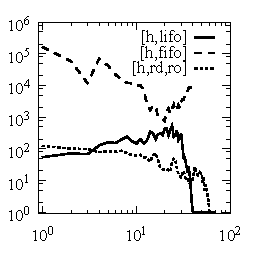
\includegraphics{tables/aaai16-log-rd/aaai16prelim3/depth-histogram-openstacks-opt11-strips-p10.pdf}
 \hfill
 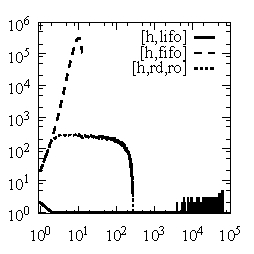
\includegraphics{tables/aaai16-log-rd/2zerocost/depth-histogram-woodworking-cut-p04.pdf}
 \hfill
 % 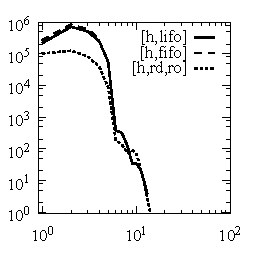
\includegraphics{tables/aaai16-log-rd/2zerocost/depth-histogram-psr-small-open-p48.pdf}
 \caption{Number of nodes ($y$-axis) expanded per depth ($x$-axis) in
 the final plateau for 
 % (in left-to-right order)
 \pddl{Openstacks} p10 
 (left)
 and
 \pddl{Woodworking-cut} p04
 (right)
 %  and
 % \pddl{psr-small-open} p48
 with different tiebreakings.
 % Axes are logarithmic.
 }
 \label{fig:depth-histogram}
\end{figure}

\subsection{Comparison With $\varepsilon$-Cost Transformation}

\begin{table}[tb]
 \centering
 \begin{tabular}{|c|c|c||c|c|}
  \hline
  Domain & $[f,h,\fifo]/\varepsilon$ &  $[f,h,\lifo]/\varepsilon$ &  $[f,h,\fd,\ro]$ &  $[f,h,\rd,\ro]$ \\
  \hline
  \lmcut Zerocost & 261 & 259 & 257.4\spm{}2.0  &  \textbf{294.2\spm{}2.3} \\
  \hline
  \mands Zerocost & 282 & 282 & 274.0\spm{}0.9  &  \textbf{310.2\spm{}2.1} \\
  \hline
 \end{tabular}
 \caption{Comparison of  depth-based tiebreaking methods vs. standard $[f,h,\fifo]$ and $[f,h,lifo]$ methods applied to $\varepsilon$-cost-transformed versions of the problem instances}
 \label{tbl:epsilon}
\end{table}

An alternative approach to addressing the large plateaus in zero-cost domains is
to eliminate plateaus by introducing artificial gradients in the search space.
For example, the cost of all zero-cost actions can be replaced by a small $\varepsilon\ll 1$, where 
$\varepsilon$ is chosen such that the optimal cost for the result of  this \emph{$\varepsilon$-cost transformation} (``$\varepsilon$-transformation'') is the same as the cost of the optimal solution to the original domain with zero costs when the $\varepsilon$-transformed costs are mapped back to 0.

We evaluated the $[f,h,\fifo]/\varepsilon$ and $[f,h,\lifo]/\varepsilon$ strategies, which are the standard $[f,h,\fifo]$ and $[f,h,\lifo]$ tiebreaking strategies applied to  the $\varepsilon$-transformed version of the problems.
Since Fast Downward  only supports integer costs, we implemented/simulated the transformation by multiplying the non-zero costs by $10^6$, and assigning cost 1 to zero-cost actions -- in effect,  $\varepsilon=10^{-6}$.
\reftbl{tbl:epsilon} shows that $[f,h,\fifo]$ and $[f,h,\lifo]$ with $\varepsilon$-transformation
 perform comparably to $[f,h,\fd,\ro]$, but are outperformed by $[f,h,\rd,\ro]$.
% 
The similarity in performance between $\varepsilon$-transformation and $[f,h,\fd,\ro]$ can be explained by the fact that  OPEN is sorted according to  $f(n)+k(n)\varepsilon$,
where $k(n)$ is a number of zero-cost actions in the path to node $n$,
while expansion order of FirstDepth is equivalent to $f(n)+\depth{n}\varepsilon$.
($\depth{n}\leq k(n)$ because $k(n)$ accounts zero-cost actions also in non-final plateaus).
% 
One advantage of the $\varepsilon$-transformation is that it can be implemented by transforming the input problem and does not require implementation of depth-based buckets in the search algorithm.
On the other hand, there are two issues with the $\varepsilon$-transformation:
(1) $\varepsilon$ must be chosen carefully -- admissibility is lost  when $k(n)\varepsilon\approx 1$, and
(2) the number of possible $g$ and $f$ values becomes very large, making it difficult to use efficient $O(1)$ array-based implementation of the OPEN list and requiring the use of a heap-based $O(\log n)$ OPEN list.
% it makes array-based $O(1)$ OPEN-list consume too much memory
% because the queue contains too many different key values, 
% or it forces
% In contrast, depth can be directly implemented with just another level of nested arrays.

\subsection{Comparison to Multi-Heuristic Tiebreaking with PLUSONE Cost Type}



\section{Related Work}
\label{sec-4}

Previous work on escaping search space plateaus has focused on
non-admissible search.  DBFS \cite{imai2011novel} % is a technique which
adds stochastic backtracking to Greedy Best First Search (GBFS) to avoid
being misdirected by the heuristic function. Type based bucket
\cite{xie14type} classifies the plateau of GBFS according to the
$[g,h]$ pair and distributes the effort.  Marvin \cite{Coles07} learns plateau-escaping macros
from the Enhanced Hill Climbing phase of the FF planner
\cite{Hoffmann01}, and the use of these macros is inadmissible.
\citeauthor{Hoffmann05} gives a detailed analysis of the
structure of the search spaces of satisficing planning (\citeyear{Hoffmann05,Hoffmann11}).
\cite{benton2010g} proposes inadmissible technique for temporal planning
where short actions 
% are hidden behind long actions and
do not increase makespan. 
\cite{cushing2010cost} investigates ``$\varepsilon$-cost
traps''($\varepsilon=\frac{\min cost}{\max cost}$),  showing that (non-admissibly) treating all actions as unit cost sometimes finds an optimal plan quickly.
\cite{wilt2011cost} also analyzes inadmissible distance-to-go estimates.
% 
To our knowledge, 
plateaus have not been previously investigated for cost-optimal planning with admissible search.
Admissible and inadmissible search differ significantly in how non-final plateaus (plateaus with $f < f^*$) are treated:
Inadmissible search can skip or escape plateaus whenever possible, while
admissible search cannot, unless it
is the final plateau ($f=f^*$, $h=0$) and a solution is found. %it directly finds a solution.

%In their work on combining multiple heuristics in a planner, 
% \citeauthor{RogerH10} (\citeyear{RogerH10}) considered a tiebreaking approach which works as follows:
% When combining two heuristics, one of the
% heuristics is used as the primary criterion, % for guiding the search,
% and the second heuristic is used to break ties among nodes with the same primary
% heuristic value.
% While this did not perform well in their work on satisficing planning, 
% additional policy using a secondary heuristic
% for cost-optimal search is an interesting direction for future work.


The PLUSONE %\footnote{This term is used on the Fast Downward website.} XXfootnote takes too much space
cost-type (or distance-to-go) is a non-admissible search technique in the Fast Downward/LAMA planner
\cite{richter2010lama} which increases all action costs by 1.
% By eliminating zero-cost actions, this behaves similar to our $[f,h,\fd,\ro]$ tiebreaking.
%Using PLUSONE, three successive
%applications of zero-cost operators have cost 3, and two
%applications have cost 2, and smaller cost is preferred, just as
%\astar always expands the node with smaller $f$-value.
This technique explicitly targeted zero-cost actions,
and resulted in significantly better performance in the IPC-6
satisficing track \cite[p.137, Sec. 3.3.2]{richter2010lama}.
%\todo*{citation}
% There's a long discussion of Openstacks in \cite{richter2010lama}, p.167-169, but I can't find PLUSONE anywhere. Maybe it's called something else in the paper?  Maybe \richter2010lama is the wrong citation??
Unlike PLUSONE, depth-based tiebreaking is admissible.
%because unlike PLUSONE, action costs are not modified.  
Also, unlike PLUSONE, depth-based tiebreaking does not necessarily favor smaller depth over larger depth.
LAMA prefers smaller cost (including the increased cost),
which biases the search toward nodes with fewer zero-cost actions on their path.
This bias is similar to the $[f,h,\fd,\ro]$ policy,
the worst performer among all depth-variants in our experiments (\reftbl{depth}).
The best depth-based methods are  $[f,h,\ld,\ro]$ and $[f,h,\rd,\ro]$,
which do not prefer smaller depth.

% It's not clear what these techniques have in common, except that they are all orthogonal to heuristics,
% If that's the case, then there's no need to cite them in this paper -- there's no reason why these particular techniques
% are more relevant to this paper than hundreds of other techniques that are orthogonal to heuristics.
%% In admissible planning,
%% \emph{Symmetry Breaking}
%% \cite{Fox1998,pochter2011exploiting,domshlak2013symmetry} is the search
%% technique that tries to prune the states with symmetric
%% paths. \emph{Partial Order Reduction}
%% % , \emph{Strong Stubborn Sets} and \emph{Expansion Core} are
%% is also a technique which prunes the
%% intermediate states that reach to the same goal using the different
%% orders of same actions. \emph{Dominance Pruning} \cite{hall2013faster} is a
%% technique which prunes a state if it can be proven to be worse than the other nodes.
%% % 
%% These are usually not considered an attempt to improve the heuristic
%% estimates, however, in terms of \emph{Path-dependent globally admissible
%% heuristics} \cite{karpas2012optimal}, a class of heuristics which is
%% admissible only on a particular optimal path, generalizes the above
%% techniques as assigning an infinite cost to some nodes on the other optimal paths.
%% % 
%% % From a slightly different category, Pathmax \cite{mero1984heuristic} and
%% % Bidirectional Pathmax \cite{felner2011inconsistent} are the techniques
%% % which converts an inconsistent heuristics into non-decreasing,
%% % consistent heuristics.
%% Thus, in a broad term, all of these methods are the
%% attempts to improve the heuristic estimates.
%% % Although in some particular
%% % case they may be able to return a perfect heuristics, they are still not
%% % always a perfect heuristics, implying that the plateau is unavoidable.
%% In contrast, our tiebreaking techniques aims specifically at the case
%% where the plateau is encountered and the planners are forced to run a
%% knowledge-free search.

%% $LA^*$ \cite{stern2010look} extends \astar by performing a
%% cost-bounded depth-first \emph{lookahead} from each node as it is generated.
%% Under the lookahead cost bound $k=0$ ($LA^*_0$ in their notation),
%% all children with the same $f$-value are expanded.
%% The tiebreaking among the same $f$ is not documented either
%% in its main $A^*$ expansion nor in its DFS lookahead.


\section{Conclusion}

In this paper, we evaluated standard tiebreaking
strategies for \astar.
We showed that contrary to conventional wisdom, tiebreaking based on the heuristic value is not necessary to achieve good performance, and proposed
a new framework for defining tiebreaking policies based on \emph{depth}.
We showed that a depth-based, randomized strategy $[f,h,\rd,\ro]$, which uses the heuristic value, but explicitly avoids depth and ordering biases present in previous methods,
significantly outperforms previous strategies on domains with zero-cost actions, 
including practical application domains with resource optimization objectives in the IPC benchmarks.
% and slightly outperforms previous strategies on benchmark problems without zero-cost actions.
%We have shown that our $[f,h,\rd,\ro]$ strategy is successful because the randomized depth bucket selection explicitly avoids the depth bias that was present in previous methods
The proposed approach is highly effective on domains where zero-cost actions create large plateau regions where all nodes have the same $f$ and $h$ costs
and the heuristic function provides no useful guidance.
% We argued that such domains arise naturally when considering resource optimization problems.
%It also avoids the effect of action ordering in the domain definition,
%providing a robust behavior.
 % when the distribution of optimal solutions is not uniform within the open list.
% We also showed that this nonuniform distribution still appears when we have almost-perfect % heuristics.
%% Our method differs from the pruning techniques because we do not prune
%% any states, nor from the other general improvements to the heuristic
%% accuracy because we just change the evaluation order within the same
%% $f$, yet it address the fundamental problems in the heuristic forward
%% search. 
%% % 


%While we focused on randomized policies because plateaus, by definition do not provide useful heuristic information, 
%a direction for future work is development of deterministic variants.

%% not much details of the idea were presented in this paper. Also, I
%% don't want it to be copied by someone;;
% on-line adaptation methods that exploit search space neighborhood structure
% in order to adjust the tiebreaking policies.

\section{Background: Tiebreaking Strategy for GBFS}

\label{sec:gbfs}

\section{Notations and Backgrounds for \\Diversified Algorithms}

We first define some notation and the terminology used throughout the
rest of the paper.
$h(s)$ denotes the heuristic estimate from the current state to the
goal state.
$g(s)$ is the current shortest path cost from the initial state to the
current state.
$f(s)=g(s)+h(s)$ is the estimate of the resulting cost of the path
containing the current state.
We omit the argument $(s)$ unless necessary.

A \emph{sorting strategy} of a best first search algorithm is a strategy
which tries to select a single node from the OPEN list.
Sorting strategies are denoted as $[\text{criterion}_1, \text{criterion}_2, ..., \text{criterion}_k]$,
which means: From the OPEN list, first, select a set of nodes using $\text{criterion}_1$.
If there are still multiple nodes remaining in the set, then break ties
using $\text{criterion}_2$ and so on,
until a single node is selected.
The \emph{first-level sorting policy} of a strategy is
$\text{criterion}_1$, the \emph{second-level sorting policy} is
$\text{criterion}_2$, and so on.
%% the word frontier is no longer used in the later text.
% \emph{final frontier} is the set of open nodes with $f^*$.
Note that this corresponds to the command line option format of Fast
Downward \cite{Helmert2006}.

Using this notation, \astar without any tiebreaking strategy can be
denoted as BFS with $[f]$, and \astar which breaks ties according to $h$
value is denoted as $[f,h]$. Similarly, GBFS is denoted as 
$[h]$.  Unless stated otherwise, we assume the nodes are sorted in the
increasing order of the key value, and a BFS always selects the smallest
key value.



The sorting strategy may fail to select a single node. In such cases, a
search algorithm must decide which node to expand by the
\emph{last-resort} tiebreaking strategy, which is one of FIFO
(First-In-First-Out), LIFO (Last-In-First-Out) or RAND (random
ordering).  Trivially, these strategies are able to select a single node
from the set of nodes.  Throughout the paper, we show the last-resort
tiebreaking in the subscript such as $[f,h]_{\lifo}$, and we imply LIFO
when it is omitted.

% A \emph{plateau} is a set of nodes in OPEN with both the same $f$ and same $h$ costs.
% A plateau whose nodes have $f$-cost $f_p$ and $h$-cost $h_p$ is denoted as
% $\plateau{f_p,h_p}$.
% An  \emph{entrance} to a $\plateau{f_p,h_p}$ is a node $n \in \plateau{f_p,h_p}$, whose current parent is not a member of $\plateau{f_p,h_p}$.
% The \emph{final plateau},  is the plateau containing the solution found by the search algorithm.
% In \astar using admissible heuristics, the final plateau is  $\plateau{f^*,0}$.

\section{Backgrounds}

\todo{unrelated -- interesting but too ambitious?}
Heuristic errors consist of two major components called \emph{precision}
and \emph{accuracy}. Both terms are defined based on the distribution of
the heuristic estimates compared to the true distance to the goal $h^*$,
but has a key difference as follows: \emph{accuracy} accounts for the
difference of means, while \emph{precision} accounts for the deviation
from the true distance. The notion was proposed in the early days of
literature for investigating the performance of probabilistic heuristic
function \cite{pearl1984heuristics}, but is largely forgotten in the
current search community. \citeauthor{pearl1984heuristics}
concluded that, for satsificing search, the key characteristics which
determines the performance of inadmissible heuristics is
\emph{precision}, rather than \emph{accuracy}. Assume we have an
inadmissible heuristic function which always overestimates the true
distance $h^*$ by a constant error $e$ --- the guidance provided by
function $h^*(s)+e$ is not much different from that of $h^*(s)$
itself. This is because it changes the accuracy but does not change
the precision of the heuristics.

KBFS(k) \cite{Korf??} is an early attempt on alleviating the problem of
GBFS. It expands $k$ nodes at a time in order to prevent the search
algorithm from getting stuck in the heuristic trap. KBFS provided an
interesting observation to GBFS --- KBFS(1) is equivalent to GBFS, and
KBFS($\infty$) is equivalent to Breadth-First Search.

Alternation OPEN List \cite{RogerH10} is a technique to combine multiple
heuristic functions during the search in order to improve the robustness
of the search algorithm. Nodes are simultaneously stored and sorted into the
multiple independent OPEN lists with different sorting strategies, and
it alternates among the OPEN lists when it expands a new node.
We denote an alternating OPEN list as $\mit{alt}(X_1,X_2,\ldots)$ where
each $X_i$ is a sorting strategy.

$\epsilon$-greedy GBFS \cite{valenzano2014comparison} is a variation of GBFS
which selects a random node in the OPEN list at a certain fixed
probability $\epsilon <1$ given as a parameter. When the random
exploration takes place, the entire nodes in OPEN list are treated equally, and
there is no explicit criteria for characterising the nodes.
This is conceptually equivalent to the weighted version of the alternation
open list using $[h]_{\fifo}$ and $[\ ]_{\ro}$ (no sorting criteria) with weights
$1-\epsilon$ and $\epsilon$. We denote such a weighted alternation open
list as $\mit{alt}(w_1X_1,w_2X_2,\ldots)$ where each $w_i$ is a weight
for a sorting strategy $X_i$. Now $\epsilon$-greedy GBFS corresponds to
$\mit{alt}((1-\epsilon)[h]_{\fifo},\epsilon [\ ]_{\ro})$.

While the exploration phase of $\epsilon$-greedy GBFS does not have any method to detect the bias
between the nodes,
Type-GBFS \cite{xie14type} does this by running the 
classification of the nodes. The nodes are categorized into buckets
(called ``type bucket''), each associated with a specific vector of key
values, such as $[g,h]$ for each state. On each explorative
expansion, the search algorithm selects a random node in a random
bucket, which avoids the cardinality bias --- the search nodes
may be more concentrated in a particular bucket, and exploration done by
$\epsilon$-greedy fails to explore the variety of search space, unlike
Type-GBFS.

Type-GBFS categorizes the nodes in type buckets, but does not sort the
buckets with the key vector. Thus, we denote such a random
selection among buckets as $\brackets{\ldots}$ where $\ldots$ is a
classification criteria, e.g., $\brackets{g,h}$ denotes the type buckets
whose keys are the vector $[g,h]$.

In their paper, the method was evaluated under a
configuration that the explorative expansion and the exploitative
expansion (standard GBFS) alternates. 
Thus, we can write this algorithm as $\mit{alt}([h], \brackets{g,h}_{\ro})$.
% This also corresponds to the case of $\epsilon$-greedy with $\epsilon=0.5$.
% 
They empirically show that
this configuration results in larger coverage and that it
expands much broader variety of nodes in the explorative
expansion phase.

\begin{table}[htbp]
 \centering
 \setlength{\tabcolsep}{0.2em}
 % \begin{tabular}{|l|l|}
 \begin{align*}
  \mbox{\astar without tiebreaking}         &: [f]   \\
  \mbox{\astar, break ties for smaller $h$} &: [f,h] \\
  \mbox{Standard GBFS}                      &: [h]   \\
  \mbox{GBFS+Alternation (2 heuristics)}    &: \mit{alt}([h_1],[h_2])   \\
  \mbox{$\epsilon$-greedy GBFS}             &: \mit{alt}((1-\epsilon)[h], \epsilon [\ ]_{\ro}) \\
  \mbox{Type-GBFS, type = $[g,h]$}          &: \mit{alt}(\quad       [h],\quad \brackets{g,h}_{\ro}) \\
  \mbox{$\epsilon$-greedy Type-GBFS}        &: \mit{alt}((1-\epsilon)[h], \epsilon\brackets{g,h}_{\ro}) \\
  \mbox{\astar + $h$ tiebreaking + depth}   &: [f,h]_{\brackets{\mit{\scriptsize depth}}} \\
  \mbox{GBFS + depth}                       &: [h]_{\brackets{\mit{\scriptsize depth}}} \\
 \end{align*}
 % \end{tabular}
 \caption{Various search algorithms using the notation in this paper}
\end{table}

%% less priority. remove?
% DBFS \cite{imai2011novel} is also an algorithm which diversifies the
% search based on $g$ and $h$ values, but with several key differences from
% above two algorithms: First, the explorative selection is not uniformly
% random, but is subject to a particular distribution function defined by
% $h, g, h_{min}$ and $g_{max}$. Second, it uses a local search with
% a bounded number of expansions equal to $h(s)$, which dynamically balances the exploration
% and exploitation --- it does more GBFS when $h$ is large (far
% from the goal), and less GBFS near the goal ($h$ is small).



% The diversification based on the depth can be considered as an instance
% of last-resort tiebreaking, since the depth is used \emph{after} the
% sorting strategy selects a set of nodes.
% % 
% We can also view the depth-based diversification as a classification of
% the nodes into type-based buckets with depth as a single key value.
% Thus, we call this framework as \emph{typed-sorting strategy}, a mix of
% sorting strategy and type-based buckets, denoted as $[\mbox{sorting
% strategy}]_{\brackets{\mbox{\small type vector}}}$.
% % 
% For example, \astar using $h$ as the first tiebreaking criteria and
% depth as a diversification method can be expressed as
% $[f,h]_{\brackets{d}}$. 
% % _{\fifo}
% % The reason \fifo is present
% % after $\brackets{d}$ is that when multiple nodes are in the same depth, a
% % single node is selected in a FIFO order.
% % Trivially, $[\ ]_{\brackets{X}}$ is equivalent to $\brackets{X}$ and
% % $[X]_{\brackets{\ }}$ is equivalent to $[X]$.


\section{Depth-based Tiebreaking for GBFS}

%\citeauthor{Korf1985depth} uses $h$-based tiebreaking in the context of WA*
%\cite{korf1993linear} 
% 
% (g-based tiebreaking, p69, for GBFS:) With all the weight on h, meaning
% that g is used only for tie-breaking among nodes with equal h values,
% 
% (p73:) to break ties in favor of nodes closest to the initial state.  
% ** not sure how/where to put this..


Compared to \astar, to our knowledge, there are currently no
well-established tiebreaking policy for GBFS. GBFS does not use $f$ and
$g$ value during the search process.  The search by GBFS is solely
guided by the heuristic value $h$: It always expands the node with the
smallest $h$ value, and hence the analogy from \astar e.g.\ sorting the
nodes with $f$ and breaking ties according to $h$ is not possible.

As a consequence, except for diversification,
search enhancement for GBFS have been achieved by
modifying the heuristic function itself.  This includes not only using the
different heuristic functions, but also lazy evaluation,
preferred operators and PLUSONE/ONE cost type.
 
Lazy evaluation is a technique which derives the heuristic value of a
state from its parent. This sacrifices the informativeness of the
heuristics against the effort of computing each heuristic function.
 
Preferred operator (helpful action in \cite{Hoffmann01}) marks some
operators to be promising when it improved the least cost estimate in the
previous node expansion. Marked nodes are put in a special queue
which is expanded more often, which is equivalent to temporarily
increasing the priority of the particular nodes.
 
PLUSONE cost type is a technique which adds a cost of 1 to each edge
cost, which also affects the heuristic value. Similarly, ONE cost type
treats all actions to have a unit cost.  ONE cost type is used in
the first GBFS iteration of LAMA, and PLUSONE cost type is used in the
second GBFS iteration of LAMA (followed by WA*).

We instead consider the use of the depth-based tiebreaking policy, which
is able to identify the relative location of the current state in the
plateau.  In this section, we evaluate the effect of depth-based
tiebreaking on Eager GBFS, and also compare the effect
against various search enhancements stated above.

\subsection{Comparison against GBFS}

We compared the performance of 
($G$) the standard GBFS
$[h]$,
($G_d$) GBFS using depth-based diversification
$[h]_{\relsize{-2}\brackets{d}}$,
($T$) Type-GBFS
$alt([h],\brackets{g,h})$,
($T_d$) Type-GBFS using depth-based diversification
$alt([h]_{\brackets{d}},\brackets{g,h})$,
($T^d$) Type-GBFS using depth-based type bucket
$alt([h],\brackets{g,h,d})$,
($T_d^d$) Type-GBFS using both depth-based diversification and depth-based type bucket
$alt([h]_{\brackets{d}},\brackets{g,h,d})$.

Since the effect of depth could be heuristic-dependent, we tested three
heuristics as $h$:
FF heuristics\cite{Hoffmann01}, Causal Graph (CG) heuristics \cite{Helmert2006}, Context Enhanced
Additive (CEA) heuristics\cite{helmert2008unifying}.
%% not included --- its is a pseudo heuristics anyways
% , Landmark-Count (LC) heuristics\cite{richter2008landmarks}



% In order to remove the effect of randomness of the algorithm, we
% implemented a deterministic version of Type-based queue for Type-GBFS
% which, instead of selecting a bucket at random, iterates over the
% buckets in a reverse order that each bucket is introduced.
% Similarly, the diversification based on the depth is not randomized but
% is implemented as a loop-based implementation.

Results are shown in \reftbl{eager-results}. Overall, depth offers
improvements to all of CEA, CG and FF heuristics. Thus, we conjecture
that the effect of depth-based diversification is heuristic-independent.

We also tested the effect of lazy (deferred) evaluation of the
heuristic functions. As explained in the previous section, lazy
evaluation can be considered as a form of modifying the heuristic
function by sacrificing the accuracy for the node expansion rate.
As expected, depth-based diversification offers the similar speedup as
in the case of eager evaluation.

Another dimension we should consider in evaluating the depth
diversification is the use of PLUSONE which treats all
action costs as the original value plus 1, or ONE cost type which treats
all actions as the unit cost.

% \newcommand{\htitle}[1]{\multicolumn{#1}{c|}{CEA} & \multicolumn{#1}{|c|}{CG} & \multicolumn{#1}{|c|}{FF}}
\newcommand{\etitle}[2]{ \multicolumn{#1}{|c||}{Eager} & \multicolumn{#1}{|c|#2}{Lazy}}
\newcommand{\htitle}[2]{\multicolumn{#1}{c|}{CEA} & \multicolumn{#1}{|c|}{CG} & \multicolumn{#1}{|c|#2}{FF}}
\newcommand{\titles}[3]{
&\etitle{#1}{#3} \\
\hline
&\htitle{#2}{|} #3 &\htitle{#2}{}\\
\hline
}

\begin{table}[htbp]
 \setlength{\tabcolsep}{0.1em}
 % \setlength{\tabcolsep}{0.05em}
 % \relsize{-1}
\centering
\begin{tabular}{|l*{2}{*{3}{|cc}|}*{2}{*{3}{|cc}|}}
\hline
&\etitle{6}{|} & \etitle{6}{}\\
\hline
&\htitle{2}{|} & \htitle{2}{|} &\htitle{2}{|} & \htitle{2}{}\\
\hline
 & g & G & g & G & g & G & g & G & g & G & g & G & gt & Gt & gt & Gt & gt & Gt & gt & Gt & gt & Gt & gt & Gt\\
\hline
coverage & 189 & \bi{193} & 174 & \bi{183} & 166 & 167 & 139 & \bi{172} & 137 & \bi{144} & 146 & \bi{162} & \bi{203} & 200 & 203 & \bi{210} & \bi{217} & 215 & 157 & \bi{173} & 165 & \bi{179} & 178 & \bi{212}\\
\hline
brmn & 0 & 0 & 0 & 0 & 0 & 0 & 0 & 0 & 0 & 0 & 1 & 0 & 0 & 0 & 0 & 0 & 0 & 1 & 0 & 0 & 0 & 0 & 0 & 0\\
lvtr & 1 & \bi{3} & 3 & \bi{5} & 0 & 0 & 1 & \bi{4} & 1 & \bi{4} & 0 & 0 & 1 & \bi{3} & 3 & 3 & 0 & 0 & 1 & \bi{3} & 1 & \bi{4} & 0 & 0\\
flrt & 4 & 4 & 0 & 0 & 7 & 7 & 6 & 6 & 0 & 0 & \bi{8} & 4 & 7 & 7 & 2 & 2 & 9 & 9 & 6 & 7 & 2 & 2 & 8 & 9\\
nmys & 7 & 7 & 7 & 7 & 6 & \bi{8} & 8 & 8 & 9 & 9 & 5 & \bi{7} & 9 & 9 & \bi{16} & 14 & 16 & 15 & 11 & 11 & 14 & 15 & 15 & 16\\
pnst & 0 & 0 & 0 & 0 & 0 & 0 & 0 & 0 & 0 & 0 & 0 & 0 & 0 & 0 & 0 & 0 & 0 & 0 & 0 & 0 & 0 & 0 & 0 & 0\\
prcp & 15 & 15 & 15 & 15 & 5 & 5 & 12 & 12 & 11 & 11 & 0 & 0 & 15 & 15 & 15 & 15 & 7 & 7 & 11 & 11 & 10 & 10 & 6 & 6\\
prkn & 0 & 1 & 12 & 13 & 15 & 14 & 2 & \bi{4} & 3 & \bi{11} & 14 & \bi{19} & 3 & 2 & 7 & \bi{9} & \bi{12} & 8 & 1 & 0 & 3 & 4 & 15 & 16\\
pgsl & 19 & 19 & 20 & 20 & 19 & 19 & 19 & 19 & 20 & 19 & 20 & 20 & 20 & 20 & 20 & 20 & 20 & 20 & 20 & 19 & 20 & 20 & 20 & 20\\
scnl & 17 & 17 & 17 & 17 & 14 & 14 & 17 & 17 & 17 & 17 & 15 & 14 & 17 & 17 & 17 & 17 & 16 & 16 & 17 & 17 & 17 & 17 & 17 & 17\\
skbn & 12 & 12 & 14 & 14 & 18 & 17 & 10 & 11 & 15 & 15 & 18 & 17 & 15 & 16 & 16 & 17 & 18 & 18 & 16 & 16 & 13 & \bi{16} & 18 & 18\\
tdyb & 16 & 17 & 14 & \bi{18} & 15 & 14 & 16 & 17 & 14 & \bi{17} & 14 & 13 & 16 & 16 & 19 & 19 & 16 & 16 & 16 & 17 & 20 & 20 & 14 & \bi{16}\\
trns & 7 & 7 & 9 & \bi{11} & 0 & 0 & 3 & \bi{5} & 7 & 8 & 0 & 0 & 7 & 7 & 11 & 11 & 0 & 0 & 4 & 5 & 9 & 8 & 0 & 0\\
vstl & 3 & 3 & 3 & 3 & 5 & 5 & 3 & 3 & 3 & 3 & 5 & 4 & 4 & 4 & 4 & 5 & 6 & 5 & 4 & 4 & 5 & 5 & 4 & \bi{6}\\
wdwr & 10 & 10 & 10 & 10 & 12 & 12 & 2 & 3 & 1 & 1 & 10 & 11 & 12 & 11 & 12 & 13 & 15 & 15 & 3 & 4 & 1 & 1 & 7 & \bi{13}\\
\hline
brmn & 0 & 0 & 0 & 0 & 0 & 0 & 0 & 0 & 0 & 0 & 0 & 0 & 0 & 0 & 0 & 0 & 3 & 2 & 0 & 0 & 0 & 0 & 0 & 0\\
cvdv & 6 & 6 & 7 & 7 & 6 & 6 & 4 & \bi{7} & 7 & 7 & 6 & 6 & 6 & 7 & 7 & 7 & 7 & 7 & 7 & 7 & 8 & 8 & 7 & 7\\
chld & 2 & 2 & 2 & 2 & 0 & 0 & 0 & 0 & 0 & 0 & 0 & 0 & \bi{2} & 0 & \bi{3} & 0 & 0 & 0 & 2 & 1 & 6 & 5 & 2 & 2\\
ctyc & 20 & 20 & 0 & \bi{2} & 0 & 0 & 1 & \bi{20} & 0 & 0 & 0 & 0 & 20 & 20 & 1 & 1 & 18 & \bi{20} & 1 & \bi{15} & 0 & 0 & 1 & \bi{10}\\
flrt & 2 & 2 & 0 & 0 & 2 & 2 & 2 & 2 & 0 & 0 & 3 & 3 & \bi{5} & 3 & 2 & 1 & \bi{5} & 3 & 3 & 2 & 2 & 2 & 3 & 3\\
gd-s & 0 & 0 & 0 & 0 & 0 & 0 & 0 & 0 & 0 & 0 & 0 & 0 & 0 & 0 & 0 & 0 & 0 & 0 & 0 & 0 & 0 & 0 & 0 & 0\\
hkng & 17 & 16 & 15 & 14 & 16 & \bi{18} & 17 & 17 & \bi{16} & 13 & 12 & \bi{14} & 16 & 16 & 20 & 20 & 20 & 20 & 16 & 15 & 18 & 19 & 18 & 18\\
mntn & 16 & 16 & 16 & 16 & 11 & 12 & 0 & 0 & 0 & 0 & 4 & \bi{7} & 16 & 16 & 16 & 16 & 13 & 14 & 7 & 7 & 7 & 7 & 9 & 10\\
pnst & 0 & 0 & 0 & 0 & 0 & 0 & 0 & 0 & 0 & 0 & 0 & 0 & 0 & 0 & 0 & 0 & 0 & 0 & 0 & 0 & 0 & 0 & 0 & 0\\
prkn & 0 & 1 & 1 & 1 & 1 & 1 & 0 & 1 & 0 & 1 & 3 & \bi{11} & 0 & 0 & 0 & 0 & 2 & 2 & 0 & 0 & 0 & 0 & 1 & \bi{8}\\
ttrs & 3 & 4 & 2 & 2 & 3 & 3 & 1 & \bi{4} & 2 & 2 & 1 & \bi{3} & 2 & 2 & 6 & \bi{12} & 2 & \bi{4} & 1 & 2 & 2 & \bi{9} & 3 & \bi{6}\\
thgh & 11 & 11 & 4 & 5 & 11 & 10 & 12 & 12 & \bi{6} & 4 & 7 & \bi{9} & 9 & 8 & 5 & 5 & 12 & 13 & 9 & 9 & 5 & 5 & 10 & 11\\
trns & 1 & 0 & \bi{3} & 1 & 0 & 0 & \bi{3} & 0 & \bi{5} & 2 & 0 & 0 & 1 & 1 & 1 & \bi{3} & 0 & 0 & 1 & 1 & 2 & 2 & 0 & 0\\
vstl & 0 & 0 & 0 & 0 & 0 & 0 & 0 & 0 & 0 & 0 & 0 & 0 & 0 & 0 & 0 & 0 & 0 & 0 & 0 & 0 & 0 & 0 & 0 & 0\\
\hline
\end{tabular}
\caption{Results of 5 min, 4Gb experiments, comparing the variants with and without depths:}%
 % (g): GBFS $[h]$,
 % (G): GBFS with depth based diversification $[h]_\{d\}$.
 % Left side shows the result of eager evaluation, and the right side shows
 % the result of lazy evaluation.
 % ,
 % (gt): $alt([h],\brackets{g,h})$,
 % (gT): $alt([h],\brackets{g,h,d})$,
 % (Gt): $alt([h]_{\brackets{d}},\brackets{g,h})$,
 % (GT): $alt([h]_{\brackets{d}},\brackets{g,h,d})$
 % }
\end{table}

\begin{table}[htbp]
\centering
\setlength{\tabcolsep}{0.1em}
\begin{tabular}{lll|ccc|ccc}
 &  &  & Eager & Eager & Eager & Lazy & Lazy & Lazy\\
 &  &  & IPC7 & IPC8 & sum & IPC7 & IPC8 & sum\\
\hline
ce & g & F & 112 & 70 & 182 & 116 & 54 & 170\\
ce & G & F & 113 & 70 & 183 & 119 & 48 & 167\\
ce & gt & F & 120 & 67 & 187 & 125 & 67 & 192\\
ce & gT & F & 120 & 67 & 187 & 125 & 66 & 191\\
ce & Gt & F & 120 & \bi{77} & 197 & 128 & 62 & 190\\
ce & GT & F & 121 & \bi{77} & 198 & 129 & 62 & 191\\
cg & g & F & 126 & 54 & 180 & 110 & 37 & 147\\
cg & G & F & 132 & 55 & 187 & 118 & 36 & 154\\
cg & gt & F & 139 & 63 & 202 & 122 & 49 & 171\\
cg & gT & F & 138 & 63 & 201 & 121 & 49 & 170\\
cg & Gt & F & \bi{142} & 63 & \bi{205} & 129 & 56 & 185\\
cg & GT & F & \bi{142} & 63 & \bi{205} & 128 & 56 & 184\\
ff & g & F & 110 & 49 & 159 & 110 & 48 & 158\\
ff & G & F & 110 & 54 & 164 & 117 & 45 & 162\\
ff & gt & F & 130 & 71 & 201 & \bi{137} & \bi{75} & \bi{212}\\
ff & gT & F & 129 & 71 & 200 & 136 & \bi{75} & 211\\
ff & Gt & F & 134 & 68 & 202 & 132 & 59 & 191\\
ff & GT & F & 135 & 70 & \bi{205} & 133 & 59 & 192\\
\hline
ce & g & L & 111 & 78 & 189 & 99 & 40 & 139\\
ce & G & L & 115 & 78 & 193 & 109 & 63 & 172\\
ce & gt & L & 126 & 77 & 203 & 110 & 47 & 157\\
ce & gT & L & 127 & 76 & 203 & 114 & 45 & 159\\
ce & Gt & L & 127 & 73 & 200 & 114 & 59 & 173\\
ce & GT & L & 125 & 75 & 200 & 116 & 54 & 170\\
cg & g & L & 124 & 50 & 174 & 101 & 36 & 137\\
cg & G & L & 133 & 50 & 183 & 115 & 29 & 144\\
cg & gt & L & 142 & 61 & 203 & 115 & 50 & 165\\
cg & gT & L & 141 & 57 & 198 & 119 & 41 & 160\\
cg & Gt & L & \bi{145} & 65 & 210 & 122 & 57 & 179\\
cg & GT & L & \bi{145} & 59 & 204 & 122 & 48 & 170\\
ff & g & L & 116 & 50 & 166 & 110 & 36 & 146\\
ff & G & L & 115 & 52 & 167 & 109 & 53 & 162\\
ff & gt & L & 135 & 82 & \bi{217} & 124 & 54 & 178\\
ff & gT & L & 127 & 79 & 206 & 130 & 46 & 176\\
ff & Gt & L & 130 & \bi{85} & 215 & 137 & \bi{75} & \bi{212}\\
ff & GT & L & 133 & 74 & 207 & \bi{140} & 70 & 210\\
\end{tabular}
\end{table}

\begin{table}[htbp]
 \setlength{\tabcolsep}{0.1em}
 % \setlength{\tabcolsep}{0.05em}
 % \relsize{-1}
\centering
\begin{tabular}{|l*{2}{*{3}{|cc}|}*{2}{*{3}{|cc}|}}
\hline
&\etitle{6}{|} & \etitle{6}{}\\
\hline
&\htitle{2}{|} & \htitle{2}{|} &\htitle{2}{|} & \htitle{2}{}\\
\hline
 % & e & e & e & e & e & e & l & l & l & l & l & l & e & e & e & e & e & e & l & l & l & l & l & l\\
 % & ce1 & ce1 & cg1 & cg1 & ff1 & ff1 & ce1 & ce1 & cg1 & cg1 & ff1 & ff1 & ce1 & ce1 & cg1 & cg1 & ff1 & ff1 & ce1 & ce1 & cg1 & cg1 & ff1 & ff1\\
 & g & G & g & G & g & G & g & G & g & G & g & G & gt & Gt & gt & Gt & gt & Gt & gt & Gt & gt & Gt & gt & Gt\\
\hline
IPC7 & 118 & 118 & 140 & \bi{143} & \bi{142} & 139 & 99 & \bi{117} & 113 & \bi{134} & 112 & \bi{143} & 130 & 130 & 153 & 154 & \bi{166} & 157 & 106 & \bi{121} & 124 & \bi{146} & 135 & \bi{156}\\
\hline
brmn & 0 & 0 & 0 & 0 & 0 & 0 & 0 & 0 & 0 & 0 & 1 & 0 & 0 & 0 & 0 & 0 & 10 & 10 & 0 & 0 & 0 & 0 & 2 & 2\\
lvtr & 8 & 8 & 8 & 9 & 10 & 10 & 10 & 10 & 9 & 8 & 8 & \bi{12} & 8 & 8 & 8 & 9 & 10 & 10 & 5 & \bi{8} & 7 & \bi{9} & 4 & \bi{11}\\
flrt & 3 & 3 & 0 & 0 & 3 & 4 & 3 & 3 & 0 & 0 & 3 & 3 & 5 & 5 & 2 & 2 & 8 & 7 & 5 & 5 & 2 & 2 & 6 & 6\\
nmys & 7 & 7 & 7 & 7 & 6 & \bi{8} & 8 & 8 & 9 & 9 & 4 & \bi{7} & 9 & 9 & \bi{16} & 14 & 16 & 15 & 11 & 11 & 14 & 15 & 15 & 16\\
pnst & 13 & 12 & 13 & 13 & 15 & 15 & 0 & \bi{15} & 0 & \bi{14} & 0 & \bi{20} & 11 & 11 & 11 & 11 & 13 & 13 & 0 & \bi{11} & 1 & \bi{12} & 4 & \bi{9}\\
prcp & 20 & 20 & 20 & 19 & 20 & 20 & 11 & 11 & 11 & 11 & 11 & 11 & 18 & 18 & 18 & 19 & 20 & 20 & 12 & 13 & 11 & 12 & 14 & 14\\
prkn & 0 & \bi{2} & 12 & 13 & \bi{15} & 11 & 2 & \bi{4} & 3 & \bi{11} & 14 & \bi{19} & 3 & 2 & 7 & \bi{9} & \bi{12} & 8 & 1 & 0 & 3 & 4 & 15 & 16\\
pgsl & 20 & 20 & 20 & 20 & 19 & 20 & 20 & 20 & 20 & 20 & 20 & 20 & 20 & 20 & 20 & 20 & 20 & 20 & 20 & 20 & 20 & 20 & 20 & 20\\
scnl & 17 & 17 & 17 & 17 & 14 & 14 & 17 & 17 & 17 & 17 & 12 & 13 & 16 & 16 & 17 & 17 & 15 & 15 & 17 & 17 & 17 & 17 & 17 & 17\\
skbn & 3 & 3 & 13 & 12 & 18 & 17 & 3 & 3 & 15 & 14 & 18 & 17 & 10 & 10 & 17 & 17 & 18 & 17 & 10 & 9 & 15 & \bi{17} & 18 & 18\\
tdyb & 16 & 17 & 14 & \bi{18} & \bi{15} & 13 & 16 & 17 & 14 & \bi{17} & 14 & 13 & 16 & 16 & 19 & 19 & 16 & 15 & 16 & 17 & 20 & 20 & 14 & \bi{16}\\
trns & \bi{7} & 5 & 12 & 11 & 0 & 0 & 4 & 5 & \bi{11} & 9 & 0 & 0 & 6 & \bi{8} & 13 & 12 & 0 & 0 & 3 & \bi{5} & 8 & \bi{12} & 0 & 0\\
vstl & 3 & 3 & 3 & 3 & 5 & 5 & 3 & 3 & 3 & 3 & 5 & 4 & 4 & 4 & 4 & 4 & 6 & 5 & 4 & 4 & 5 & 5 & 4 & \bi{6}\\
wdwr & 1 & 1 & 1 & 1 & 2 & 2 & 2 & 1 & 1 & 1 & 2 & \bi{4} & 4 & 3 & 1 & 1 & 2 & 2 & 2 & 1 & 1 & 1 & 2 & \bi{5}\\
\hline
IPC8 & 62 & 62 & 60 & \bi{64} & 73 & 73 & 36 & \bi{50} & 39 & \bi{48} & 54 & \bi{93} & \bi{57} & 55 & 76 & \bi{79} & 80 & 79 & 44 & \bi{53} & 66 & \bi{74} & 66 & \bi{92}\\
\hline
brmn & 0 & 0 & 0 & 0 & 0 & 0 & 0 & 0 & 0 & 0 & 0 & 0 & 0 & 0 & 0 & 0 & \bi{4} & 2 & 0 & 0 & 0 & 0 & 0 & 0\\
cvdv & 6 & 6 & 7 & 7 & 7 & 7 & 4 & \bi{7} & 7 & 7 & 6 & 7 & 6 & 6 & 7 & 7 & 7 & 7 & 6 & 7 & 7 & 8 & 7 & 7\\
chld & 2 & 2 & 2 & 2 & 0 & 0 & 0 & 0 & 0 & 0 & 0 & 0 & \bi{2} & 0 & \bi{3} & 0 & 0 & 0 & 2 & 1 & 6 & 5 & 2 & 2\\
ctyc & 2 & 2 & 0 & 1 & 0 & 0 & 0 & \bi{2} & 0 & 0 & 0 & 0 & 4 & 5 & 1 & 1 & 3 & 3 & 1 & \bi{9} & 0 & 0 & 0 & \bi{7}\\
flrt & 2 & 2 & 0 & 0 & 2 & 2 & 2 & 2 & 0 & 0 & 2 & 2 & 2 & 2 & 2 & 2 & 2 & 2 & 2 & 2 & 1 & 1 & 2 & 2\\
gd-s & 0 & 0 & 0 & 0 & \bi{19} & 17 & 0 & 0 & 0 & 0 & 20 & 20 & 0 & 0 & 8 & 9 & 16 & 15 & 0 & 0 & 11 & 11 & 15 & \bi{17}\\
hkng & 17 & 16 & 15 & 14 & 16 & \bi{18} & 17 & 17 & \bi{16} & 13 & 12 & \bi{14} & 16 & 16 & 20 & 20 & 20 & 20 & 16 & 15 & 18 & 19 & 18 & 18\\
mntn & 16 & 16 & 16 & 16 & 11 & 12 & 0 & 0 & 0 & 0 & 4 & \bi{7} & 16 & 16 & 16 & 16 & 13 & 13 & 7 & 7 & 7 & 7 & 9 & 10\\
pnst & 0 & 0 & 0 & 0 & 4 & 4 & 0 & \bi{3} & 0 & \bi{3} & 0 & \bi{20} & 0 & 0 & 0 & 0 & 0 & 0 & 0 & 0 & 0 & 1 & 0 & \bi{6}\\
prkn & 0 & 2 & 1 & 1 & 2 & 1 & 0 & 1 & 0 & 1 & 3 & \bi{11} & 0 & 0 & 0 & 0 & 1 & 2 & 0 & 0 & 0 & 0 & 1 & \bi{8}\\
ttrs & 4 & 3 & 12 & \bi{15} & 1 & 2 & 1 & \bi{5} & 7 & \bi{17} & 0 & \bi{3} & 1 & 1 & 13 & \bi{15} & 2 & 2 & 1 & 3 & 9 & \bi{15} & 2 & \bi{4}\\
thgh & 12 & 11 & 4 & 5 & 11 & 10 & 12 & 12 & \bi{6} & 4 & 7 & \bi{9} & 9 & 8 & 5 & 5 & 12 & 13 & 9 & 9 & 5 & 5 & 10 & 11\\
trns & 1 & 2 & 3 & 3 & 0 & 0 & 0 & 1 & 3 & 3 & 0 & 0 & 1 & 1 & 1 & \bi{4} & 0 & 0 & 0 & 0 & 2 & 2 & 0 & 0\\
vstl & 0 & 0 & 0 & 0 & 0 & 0 & 0 & 0 & 0 & 0 & 0 & 0 & 0 & 0 & 0 & 0 & 0 & 0 & 0 & 0 & 0 & 0 & 0 & 0\\
\hline
\end{tabular}
\caption{Results obtained by treating each action to have a unit cost
 during heuristic calculation.
 5 min, 4Gb experiments, comparing the variants with
 and without depths:
 % (g): GBFS $[h]$,
 % (G): GBFS with depth based diversification $[h]_\brackets{d}$.
 Left side shows the result of eager evaluation, and the right side shows
 the result of lazy evaluation.
 % ,
 % (gt): $alt([h],\brackets{g,h})$,
 % (gT): $alt([h],\brackets{g,h,d})$,
 % (Gt): $alt([h]_{\brackets{d}},\brackets{g,h})$,
 % (GT): $alt([h]_{\brackets{d}},\brackets{g,h,d})$
 }
\end{table}


% \subsection{Comparison against Lazy Evaluation}

% Although the policy was originally designed for optimising
% \astar search with admissible heuristics, the core idea of depth would
% not be much affected by the difference between \astar and GBFS.

\subsection{Comparison against LAMA}

LAMA \cite{richter2010lama} is a \sota planner which is a winner of
IPC2011. It has numerous search enhancements including Lazy Evaluation,
Multi-heuristic search, Preferred Operators and PLUSONE cost type.

LAMA runs a GBFS followed by WA* with decreasing weights, and works in
an anytime fasion. However, this is due to the context of the
competition setting where the task also includes finding a better plan.
Since this paper focuses on GBFS, we only consider 
the coverage within the resource constraint. Thus, in the following
experiments, we do not run the successive iterations of WA* in LAMA.

The first iteration (GBFS) of LAMA is expressed as
$alt([\mit{ff}],\pref{[\mit{ff}]},[\mit{lc}],\pref{[\mit{lc}]})$, where $\mit{ff}$
denotes the FF heuristics, $\mit{lc}$ denotes the Landmark-Count heuristics,
and $\pref{X}$ denotes the preferred operator queue with sorting
strategy $X$.

We compare this base LAMA with the type-based version of LAMA and their
variants using depths.
We followed the best configuration suggested by \citeauthor{xie14type} (\citeyear{xie14type})
for Type-GBFS, which uses the type vector $\brackets{g,\mit{ff}}$.
Due to the multiple enhancements, the configurations are fairly complicated:

\begin{eqnarray}
  alt([\mit{ff}],\pref{[\mit{ff}]},[\mit{lc}],\pref{[\mit{lc}]},\brackets{g,\mit{ff}}) \\
  alt([\mit{ff}]_\brackets{d},\pref{[\mit{ff}]_\brackets{d}},[\mit{lc}]_\brackets{d},\pref{[\mit{lc}]_\brackets{d}},\brackets{g,\mit{ff}}) \\
  alt([\mit{ff}],\pref{[\mit{ff}]},[\mit{lc}],\pref{[\mit{lc}]},\brackets{g,\mit{ff},d}) \\
  alt([\mit{ff}]_\brackets{d},\pref{[\mit{ff}]_\brackets{d}},[\mit{lc}]_\brackets{d},\pref{[\mit{lc}]_\brackets{d}},\brackets{g,\mit{ff},d}) 
\end{eqnarray}

% _\brackets{d}

\begin{table}[htbp]
 \setlength{\tabcolsep}{0.2em}
\centering
\begin{tabular}{l|cccc||cccc}
 & F & F & F & F & L & L & L & L\\
 & g & G & gt & Gt & g & G & gt & Gt\\
\hline
IPC7 & \bi{223} & 220 & 224 & 224 & 210 & \bi{214} & \bi{224} & 219\\
\hline
brmn & 15 & 16 & 16 & 16 & 15 & 14 & \bi{16} & 14\\
lvtr & 14 & \bi{17} & 16 & 17 & 18 & 18 & 16 & \bi{18}\\
flrt & 3 & 2 & 4 & 4 & 3 & 3 & 4 & 4\\
nmys & 11 & 10 & 12 & 12 & 6 & \bi{9} & \bi{12} & 8\\
pnst & 20 & 20 & 20 & 20 & 20 & 20 & 20 & 20\\
prcp & \bi{20} & 18 & 16 & 17 & 14 & 14 & 16 & \bi{18}\\
prkn & 20 & 20 & 20 & 20 & 20 & 20 & 20 & 20\\
pgsl & 20 & 19 & 20 & 20 & 20 & 20 & 20 & 20\\
scnl & 17 & 17 & 17 & 17 & 17 & 17 & 17 & 17\\
skbn & 16 & 15 & 16 & 16 & 15 & 15 & 16 & 17\\
tdyb & 16 & 15 & \bi{17} & 15 & 13 & 14 & \bi{17} & 13\\
trns & 11 & 11 & 10 & 10 & 10 & 10 & 10 & 10\\
vstl & 20 & 20 & 20 & 20 & 20 & 20 & 20 & 20\\
wdwr & 20 & 20 & 20 & 20 & 19 & 20 & 20 & 20\\
\hline
IPC8 & 111 & \bi{125} & 112 & \bi{117} & 111 & \bi{121} & 114 & \bi{120}\\
\hline
brmn & 8 & \bi{10} & 9 & 8 & \bi{9} & 6 & 9 & 8\\
cvdv & 7 & 7 & 6 & 7 & 6 & 7 & 6 & 6\\
chld & 0 & \bi{10} & 2 & \bi{6} & 3 & 3 & 2 & 3\\
ctyc & 1 & 0 & 5 & 4 & 2 & \bi{4} & 5 & 5\\
flrt & 2 & 2 & 2 & 2 & 2 & 2 & 2 & 2\\
gd-s & 20 & 20 & 20 & 20 & 20 & 20 & 20 & 20\\
hkng & 15 & \bi{17} & 15 & 15 & 14 & 15 & 15 & 16\\
mntn & 1 & 1 & 6 & 6 & 1 & 1 & 6 & 7\\
pnst & 17 & 17 & 15 & \bi{17} & 16 & \bi{18} & 16 & 15\\
prkn & 9 & 9 & 6 & 6 & 9 & 10 & 7 & 8\\
ttrs & 2 & 2 & 2 & 1 & 2 & \bi{4} & 2 & 2\\
thgh & 14 & 15 & 14 & 15 & 13 & \bi{15} & 14 & \bi{17}\\
trns & 2 & 2 & 1 & \bi{3} & 2 & 3 & 1 & 1\\
vstl & 13 & 13 & \bi{9} & 7 & 12 & 13 & 9 & 10\\
\hline
\end{tabular}
\caption{Lama results.}
\end{table}



\section{Related Work}

\cite{schulte2014balancing}

\cite{auer2002finite}
